%%%%%%%%%%%%%%%%%%%%%%%%%%%%%%%%%%%%%%%%%%%%%%%%%%%%%%%%%%%%%%%%%%%%%%
% Lớp 12 | Phương trình mặt phẳng, đường thẳng, mặt cầu | Phương trình đường thẳng trong không gian
% Dạng 2H5?2-5: Vị trí tương đối giữa đường thẳng và mặt phẳng
% Số câu: 45  (sinh tự động bởi tach_cau.py; từ nay thầy sửa trực tiếp file này)
%%%%%%%%%%%%%%%%%%%%%%%%%%%%%%%%%%%%%%%%%%%%%%%%%%%%%%%%%%%%%%%%%%%%%%

%%%%%%%%%%%%%%%% TRẮC NGHIỆM 4 PHƯƠNG ÁN %%%%%%%%%%%%%%%%

% nguồn: Phan1_Lop_12_Hinh_hoc_Chuong_5
\begin{ex}%[2H5H2-5]%[ma:75a96789]
	Cho tứ diện $OABC$ có $OA, OB, OC$ đôi một vuông góc và $OA = OB  = 2a$, $OC = a\sqrt{2}$. Khoảng cách từ điểm $O$ đến mặt phẳng $(ABC)$ bằng
	 \choice
		{\True  $a$}
		{$a\sqrt{2}$} 
		 {$\dfrac{a}{2}$}
		{$\dfrac{3a}{4}$} 
	\loigiai{ 
		 Chọn hệ trục tọa độ $Oxyz$ sao cho
		$O (0;0;0)$, $ A(0;0;2a)$,  $ B(2a;0;0)$, $ C\left(0;a\sqrt{2};0\right)$.
		\begin{center}
			\tdplotsetmaincoords{70}{110} 
			\begin{tikzpicture}[scale=1.5,tdplot_main_coords,line join=round]
					\coordinate (O) at  (0,0,0);
					\coordinate (A) at  (0,0,3);
					\coordinate  (B) at (3,0,0);
					\coordinate (C) at (0,3,0); 
					\coordinate  (H) at (1,1,1);
					\coordinate (I) at (intersection cs: first line={(C)--(H)},second  line={(A)--(B)});
					\draw (A) -- (B)  -- (C) -- cycle;
					\draw[dashed] (O) -- (A); 
					\draw[dashed] (O) --  (B);
					\draw[dashed] (O) --  (C);
					\draw  (C) -- (I);
					\draw[dashed] (A) -- (I)  -- (O);
					 \draw[dashed] (B) -- (I);
					\filldraw (O) circle (1pt)  node[below] {$O$};
					\filldraw (A) circle (1pt) node[right]  {$A$};
					\filldraw (B)  circle (1pt) node[left] {$B$};
					\filldraw (C) circle (1pt) node[above  right] {$C$};
					 \filldraw (H) circle (1pt) node[below] {$H$};
					 \draw[->] (A) -- (0,0,4) node[above] {$z$};
					 \draw[->] (B) -- (4,0,0) node[left] {$x$};
					\draw[->] (C)  -- (0,4,0) node[right] {$y$};
				\end{tikzpicture}
		\end{center}
		Phương  trình mặt phẳng $(ABC)$
		$$ 
		\dfrac{x}{2a} + \dfrac{y}{a\sqrt{2}} + \dfrac{z }{2a} = 1 \Rightarrow  x + \sqrt{2}y + z - 2a = 0.
		 $$
		Khoảng cách từ  điểm $O(0;0;0)$ đến mặt phẳng $(ABC)$
		 $$
		\mathrm{d}(O, (ABC)) = \dfrac{\left|0 + \sqrt{2}\cdot 0 + 0 - 2a\right|}{\sqrt{1^2 + (\sqrt{2})^2  + 1^2}} = \dfrac{2a}{\sqrt{4}} = a.
		$$ 
	 }
\end{ex}

% nguồn: Phan1_Lop_12_Hinh_hoc_Chuong_5
\begin{ex}%[2H5H2-5]%[ma:1041fa0e]
	Trong không gian với hệ trục $Oxyz$, $M(a;b;c)$ là giao điểm của mặt phẳng $(P)\colon x + 2y -  z + 2 = 0$ và đường thẳng $d\colon \dfrac{x - 1}{2} = \dfrac{y}{-1} = \dfrac{z}{1}$. Khi đó
	 \choice
		{\True $a + b + c = -1$} 
		{$a  + b + c = 2$}
		{$a  + b + c = -2$}
		{$a + b + c = 7$} 
	 \loigiai{
		Đường thẳng $d$ có dạng tham số $\heva{&x=1+2t\\&y=-t\\&  z=t.}$\\
		Thay vào  mặt phẳng
		 \[
		(1 + 2t) + 2(-t) - t + 2 = 0 \Rightarrow 1 + 2t - 2t - t + 2 = 0\Rightarrow t =  3.
		\] 
		Khi đó $M(1 +  6, -3, 3) = (7, -3, 3)$. Vậy $a+b+c=7$.
	 }
\end{ex}

% nguồn: Phan1_Lop_12_Hinh_hoc_Chuong_5
\begin{ex}%[2H5H2-5]%[ma:2c1f3b08]
	Trong không gian với hệ tọa độ $Oxyz$, cho hai mặt phẳng 
	 $
	(P)\colon 4x - 4y + 2z  - 1 = 0$ và $(Q)\colon 2x - 2y + z + 1 = 0$
	chứa hai mặt của hình lập phương.  Thể tích khối lập phương đó bằng
	 \choice
		{$V  = \dfrac{1}{27}$}
		{\True $V =  \dfrac{1}{8}$}
		{$V =  \dfrac{1}{3\sqrt{3}}$}
		 {$V = \dfrac{1}{2\sqrt{2}}$}
	\loigiai{ 
		Giả sử hai mặt phẳng $(P)$ và $(Q)$ là hai mặt  đối của hình lập phương.\\
		 Ta thấy $
		(P) \parallel (Q)$.\\ 
		Lấy điểm $M(0;0;-1) \in (Q)$. Gọi $a$ là độ dài cạnh  của hình lập phương. Khi đó
		 $$
		a  = \mathrm{d}(M, (P)) = \dfrac{\left|4\cdot 0 - 4\cdot 0 + 2\cdot (-1) - 1\right|}{\sqrt{4^2 + (-4)^2 + 2^2}} = \dfrac{|-3|}{\sqrt{16 + 16 + 4}} = \dfrac{3}{\sqrt{36}} = \dfrac{1}{2}.
		$$ 
		 Do đó
		 $$
		V = a^3 = \left( \dfrac{1}{2} \right)^3 =  \dfrac{1}{8}.
		 $$
	} 
\end{ex}

% nguồn: Phan1_Lop_12_Hinh_hoc_Chuong_5
\begin{ex}%[2H5H2-5]%[ma:26029c65]
	Trong không gian $Oxyz$, cho đường thẳng $d\colon \heva{&x=1-t\\&y=2+2t\\&z=3+t}$ và mặt phẳng $(P)\colon x-y+3=0$. Tính số đo góc giữa đường  thẳng $d$ và mặt phẳng $(P)$.
	 \choice
		 {$120^{\circ}$}
		{$45^{\circ}$} 
		{\True  $60^{\circ}$}
		{$30^{\circ}$} 
	 \loigiai{
		Đường thẳng $d$ có véc-tơ chỉ phương $\overrightarrow{u}=(-1;2;1)$ và mặt  phẳng $(P)$ có véc-tơ pháp tuyến $\overrightarrow{n}=(1;-1;0)$. Khi đó
		$$\sin (d,(P))=\dfrac{|-1\cdot 1+2\cdot (-1)+0|}{\sqrt{1+4+1}\cdot \sqrt{1+1+0}}=\dfrac{\sqrt{3}}{2}\Rightarrow  (d,(P))=60^\circ.$$
	} 
\end{ex}

% nguồn: Phan1_Lop_12_Hinh_hoc_Chuong_5
\begin{ex}%[2H5H2-5]%[ma:f2eea2d8]
	Cho hình lập phương $ABCD.EFGH$ có cạnh bằng  $4$. Gọi $d$ là đường thẳng đi qua trọng tâm của tứ diện $EABD$, cắt đường thẳng $AE$ tại $M$ và song song với mặt phẳng $(EBD)$. Tính $AM$.
	 \choice
		{$AM = 1$} 
		{$AM =  2$}
		{\True  $AM = 3$}
		 {$AM = 4$}
	\loigiai{ 
		Chọn hệ trục tọa  độ như hình vẽ.
		\begin{center}
			\begin{tikzpicture}[scale=1,line cap=round,line join=round,font=\footnotesize,>=stealth]
					 \path
						(0,0)  coordinate (A)
						 ($(A)+(-150:1.5)$) coordinate (B)
						($(A)+(-150:2.5)$)  coordinate (x)
						($(A)+(0:2)$)  coordinate (D)
						($(A)+(0:3.5)$) coordinate  (y)
						 ($(B)+(D)-(A)$) coordinate (C)
						 ($(A)+(90:2)$) coordinate (E)
						($(D)+(90:2)$)  coordinate (H)
						($(C)+(90:2)$) coordinate  (G)
						($(B)+(90:2)$) coordinate  (F)
						($(A)+(90:3)$) coordinate (z); 
					\draw  (B)--(C)--(D)--(H)--(G)--(F)--(B)
						(G)--(C) 
						(G)--(F) 
						 (H)--(E)--(F);
					 \draw[dashed] (B)--(A)--(D)
						 (A)--(E);
					 \draw[->] (B)--(x) node[below]{$x$};
					 \draw[->] (D)--(y) node[below]{$y$};
					\draw[->] (E)--(z)  node[left]{$z$};
					\foreach \p/\r in  {A/150,D/60,C/-90,B/160,H/90,G/-50,F/180,E/150}
					\fill (\p)  circle (1.25pt) node[shift={(\r:3mm)}]{$\p$};
				\end{tikzpicture}
		\end{center}
		Ta có $A(0;0;0)$; $B(4;0;0)$; $D(0;4;0)$; $E(0;0;4)$.\\ 
		Gọi $T$ là trọng tâm của tứ diện $EABD$ suy ra $T(1;1;1)$.\\ 
		Phương trình mặt  phẳng $(EBD) \colon
		\dfrac{x}{4} + \dfrac{y}{4} + \dfrac{z}{4}  = 1 \Leftrightarrow x + y + z - 4 = 0.$\\
		Đường thẳng $d$ cắt đường thẳng $AE$ tại $M$  suy ra $M(0;0;m)$.\\
		Khi đó, $\vec{MT} = (1;1;1 - m)$ và vectơ pháp tuyến của mặt phẳng $(EBD)$  là $\vec{n} = (1;1;1)$.\\
		Do $d \parallel (EBD)$ nên $\vec{MT} \cdot \vec{n} = 0 \Leftrightarrow 1 + 1 + 1 - m = 0  \Leftrightarrow m = 3$.\\
		 Suy ra $M(0;0;3)$ nên $AM = 3$.
	} 
\end{ex}

% nguồn: Phan1_Lop_12_Hinh_hoc_Chuong_5
\begin{ex}%[2H5H2-5]%[ma:452edcae]
	Với giá trị nào của $m$ thì đường thẳng $d\colon \dfrac{x+1}{2}=\dfrac{y-3}{m}=\dfrac{z-1}{m-2}$ vuông  góc với mặt phẳng $(P)\colon x+3y+2z=2$?
	\choice 
		 {$5$}
		{$-7$} 
		{$1$} 
		{\True $6$} 
	 \loigiai{
		Một vectơ chỉ phương  của $d$ là $\overrightarrow{a}=(2;m;m-2)$ ($m\ne0$ và $m\ne2$).\\
		Một vectơ  pháp tuyến của $(P)$ là $\overrightarrow{n}=(1;3;2)$.\\
		Ta có $d\perp(P)$ nên $\overrightarrow{a}$ và $\overrightarrow{n}$ cùng phương, điều này  tương đương\\
		$$\dfrac{2}{1}=\dfrac{m}{3}=\dfrac{m-2}{2} \Leftrightarrow \heva{&m-2=4\\&m=6} \Leftrightarrow m=6.$$ 
	 }
\end{ex}

% nguồn: Phan1_Lop_12_Hinh_hoc_Chuong_5
\begin{ex}%[2H5H2-5]%[ma:9fa1fa34]
	Trong không gian với hệ trục tọa độ  $Oxyz$, cho hai đường thẳng $d\colon \dfrac{x-1}{1} = \dfrac{y-2}{-1} = \dfrac{z-3}{-1}$ và $d'\colon \dfrac{x}{2} = \dfrac{y+1}{-2} = \dfrac{z-5}{-2}$. Chọn khẳng định \textbf{đúng}.
	 \choice
		 {$d$ cắt $d'$}
		{$d$ và $d'$ chéo  nhau}
		{\True $d$ song song với $d'$} 
		{$d$  trùng với $d'$}
	 \loigiai{
		Đường thẳng $d$ và $d'$ lần lượt có vectơ chỉ phương là $\overrightarrow{u}_d=(1;-1;-1)$, $\overrightarrow{u}_{d'}=(2;-2;-2)$.\\ 
		 Vì $\overrightarrow{u}_{d'}=2\overrightarrow{u}_d$ nên $d\parallel d'$ hoặc $d\equiv d'$.\\
		Mặt khác, lấy $M(1;2;3)\in d$, thay  tọa độ $M$ vào phương trình $d'$ thấy không thỏa mãn.\\
		 Vậy $d$ song song $d'$.
	} 
\end{ex}

% nguồn: Phan1_Lop_12_Hinh_hoc_Chuong_5
\begin{ex}%[2H5V2-5]%[ma:73eab597]
	Trong không gian với hệ tọa độ $Oxyz$, cho đường thẳng $d  \colon \dfrac{x+1}{2}=\dfrac{y-1}{1}=\dfrac{z-2}{3}$ và mặt phẳng $(P) \colon x-y-z-1=0$. Phương trình đường thẳng $\Delta$ đi qua điểm $A(1;1;-2)$, song song với $(P)$ và cắt $d$ là
	 \choice
		 {$\dfrac{x-1}{1}=\dfrac{y-1}{-1}=\dfrac{z+2}{-1}$}
		 {$\dfrac{x-1}{2}=\dfrac{y-1}{1}=\dfrac{z+2}{3}$}
		{\True $\dfrac{x-1}{8}=\dfrac{y-1}{3}=\dfrac{z+2}{5}$} 
		 {$\dfrac{x-1}{2}=\dfrac{y-1}{1}=\dfrac{z+2}{1}$}
	\loigiai{ 
		Gọi $M=d \cap \Delta \Rightarrow M(-1+2t;1+t;2+3t)$.  \\
		Vectơ  chỉ phương của $\Delta$ là $\overrightarrow{AM}=(2t-2;t;3t+4)$. \\
		 Do $\Delta \parallel (P)$ nên $\overrightarrow{AM} \perp \overrightarrow{n}_P \Rightarrow 2t-2-t-3t-4=0 \Rightarrow t=-3$. \\
		Suy ra $\overrightarrow{AM}=(-8;-3;-5)$. \\ 
		Chọ $\overrightarrow{u}=-\overrightarrow{AM}=(8;3;5)$ là một vectơ chỉ phương của $\Delta$.  \\
		Vậy phương trình $\Delta \colon  \dfrac{x-1}{8}=\dfrac{y-1}{3}=\dfrac{z+2}{5}$.
	} 
\end{ex}

% nguồn: Phan1_Lop_12_Hinh_hoc_Chuong_5
\begin{ex}%[2H5V2-5]%[ma:274c4b66]
	Trong không gian $Oxyz$, cho đường thẳng $\Delta$ là giao tuyến của hai mặt phẳng $(P)\colon z-1=0$ và $(Q)\colon x+y+z-3=0$. Gọi $d$ là đường thẳng nằm trong $(P)$, cắt đường thẳng $\dfrac{x-1}{1}=\dfrac{y-2}{-1}=\dfrac{z-3}{-1}$ và vuông góc với  $\Delta$. Phương trình của $d$ là
	\choice 
		{$\heva{&x=3+t\\&y=t\\&z=1+t}$} 
		{$\heva{&x=3-t\\&y=t\\&z=1}$} 
		 {\True $\heva{&x=3+t\\&y=t\\&z=1}$}
		{$\heva{&x=3+t\\&y=-t\\&z=1+t}$} 
	 \loigiai{
		\begin{center}
			\begin{tikzpicture}
					 \path
						(0,0)  coordinate (a)
						(6,0) coordinate  (b)
						(5,2) coordinate (c) 
						(-1,2) coordinate  (d)
						(1,-1) coordinate  (e)
						(0,3) coordinate  (f) node[above]{$\Delta$}
						 (intersection of e--f and a--b) coordinate (g)
						(intersection of e--f and c--d) coordinate  (h)
						(g)--++(40:5) coordinate  (i)
						 (h)--++(40:5) coordinate (k)
						(intersection of c--d and g--i)  coordinate (l)
						 ($(g)!1/3!(h)$) coordinate (m)
						($(m)!6!90:(g)$) coordinate (o) node[right]{$d$} 
						(intersection of m--o and  g--i) coordinate (p)
						(3,6) node[left]{$d'$} coordinate (q)--++(-80:2) coordinate  (r)--++(-80:4) coordinate (s)
						(intersection of q--s and  g--i) coordinate (t)
						(intersection of m--o and  q--s) coordinate (I);
					\fill (I)  circle (1.2pt) node[above right]{$I$};
					 \draw
						 (a)--(b)--(c)--(l)
						(h)--(d)--(a) 
						 (g)--(i)--(k)--(h)--cycle
						(e)--(f) 
						 (p)--(o)
						 (q)--(r)
						 (t)--(I);
					\draw[dashed] 
						(l)--(h) 
						(m)--(p) 
						 (r)--(t)
						 (I)--(s);
					\draw pic[draw,"$P$",angle  radius=7mm] {angle=c--b--a};
					\draw  pic[draw,"$Q$",angle radius=7mm] {angle=k--i--g};
					\draw pic[draw,angle radius=3mm] {right  angle=g--m--o};
				\end{tikzpicture}
		\end{center}
		Pháp tuyến của $(P)$ là $\overrightarrow{n}_{P}=(0;0;1)$, của $(Q)$ là  $\overrightarrow{n}_{Q}=(1;1;1)$.\\
		Vì $\Delta=(P)\cap(Q)$ nên  $\overrightarrow{u}_{\Delta}=\left[\overrightarrow{n}_{P},\overrightarrow{n}_{Q}\right]=(-1;1;0)$.\\
		Đường thẳng $d\subset (P)$ và $d\perp\Delta$ nên  $\overrightarrow{n}_{d}=[\overrightarrow{n}_{P},\overrightarrow{u}_{\Delta}]=(-1;-1;0)$.\\
		Gọi $d'\colon\dfrac{x-1}{1}=\dfrac{y-2}{-1}=\dfrac{z-3}{-1}$,  đặt $A=d'\cap (P)$.\\
		Giải  hệ $\heva{&z-1=0\\&\dfrac{x-1}{1}=\dfrac{y-2}{-1}=\dfrac{z-3}{-1}}$ được $A(3;0;1)$.\\
		Vậy $d\colon\heva{&x=3+t\\&y=t\\&z=1.}$ 
	 }
\end{ex}

% nguồn: Phan1_Lop_12_Hinh_hoc_Chuong_5
\begin{ex}%[2H5V2-5]%[ma:5badacaa]
	Trong không gian với hệ tọa độ $Oxyz$, cho mặt phẳng $(P) \colon x+2y+z-4=0$ và đường thẳng $d \colon \dfrac{x+1}{2}=\dfrac{y}{1}=\dfrac{z+2}{3}$. Phương trình  đường thẳng $\Delta$ nằm trong mặt phẳng $(P)$, đồng thời cắt và vuông góc với đường thẳng $d$ là
	 \choice
		{\True $\dfrac{x-1}{5}=\dfrac{y-1}{-1}=\dfrac{z-1}{-3}$} 
		{$\dfrac{x-1}{5}=\dfrac{y-1}{1}=\dfrac{z-1}{-3}$} 
		{$\dfrac{x-1}{5}=\dfrac{y+1}{-1}=\dfrac{z-1}{2}$} 
		{$\dfrac{x+1}{5}=\dfrac{y+3}{-1}=\dfrac{z-1}{3}$} 
	\loigiai{ 
		Vectơ pháp tuyến của mặt phẳng $(P)$ là $\vec{n}_{P}=(1;2;1)$.  \\
		Vectơ chỉ  phương của đường thẳng $d$ là $\vec{u}_d=(2;1;3)$. \\
		Phương trình  tham số của đường thẳng $d\colon\heva{&x=-1+2t\\ &y=t\\ &z=-2+3t}$. \\
		Xét phương trình $-1+2t+2t-2+3t-4=0\Leftrightarrow 7t-7=0\Leftrightarrow  t=1$.\\
		Suy ra giao điểm của đường thẳng $d$ và mặt  phẳng $(P)$ là $A(1;1;1)$. Ta có $A\in\Delta$. \\
		Vectơ  chỉ phương của đường thẳng $\Delta$ là $\vec{u_\Delta}=\left[\vec{n_P},\vec{u_d}\right]=(5;-1;-3)$. \\
		 Phương trình chính tắc của đường thẳng $\Delta \colon$ $\dfrac{x-1}{5}=\dfrac{y-1}{-1}=\dfrac{z-1}{-3}$.
	} 
\end{ex}

% nguồn: Phan1_Lop_12_Hinh_hoc_Chuong_5
\begin{ex}%[2H5V2-5]%[ma:cdbb4e00]
	Trong không gian với hệ toạ độ $Oxyz$, cho hai đường thẳng $d \colon \heva{&x=2-t \\ &y=1+2t \\ &z=4-2t}$ và $d' \colon \dfrac{x-4}{1}=\dfrac{y+1}{-2}=\dfrac{z}{2}$. Phương trình nào dưới đây là phương trình đường thẳng thuộc mặt phẳng chứa $d$ và $d'$ đồng thời cách đều hai  đường thẳng đó?
	\choice 
		 {$\dfrac{x-2}{3}=\dfrac{y-1}{1}=\dfrac{z-4}{-2}$}
		{$\dfrac{x+3}{1}=\dfrac{y+2}{-2}=\dfrac{z+2}{2}$} 
		{\True  $\dfrac{x-3}{1}=\dfrac{y}{-2}=\dfrac{z-2}{2}$}
		{$\dfrac{x+3}{-1}=\dfrac{y-2}{2}=\dfrac{z+2}{-2}$} 
	\loigiai{ 
		 Đường thẳng $d$ qua $A(2;1;4)$ có vectơ chỉ phương $\overrightarrow{u}_1=(-1;2;-2)$. \\
		Đường thẳng $d'$ qua $B(4;-1;0)$ có vectơ  chỉ phương $\overrightarrow{u}_2=(1;-2;2)$. \\
		Vì $\overrightarrow{u}_1=-\overrightarrow{u}_2$ và $A \notin d'$  nên $d \parallel d'$. \\
		Đường thẳng $\Delta$ cách đều $d$ và $d'$ nên $\Delta$ đi qua trung điểm $I(3,0,2)$ của $AB$ và có một  vectơ chỉ phương $\overrightarrow{u}=(1,-2,2)$. \\
		 Phương trình $\Delta \colon$ $\dfrac{x-3}{1}=\dfrac{y}{-2}=\dfrac{z-2}{2}$.
	} 
\end{ex}

% nguồn: Phan1_Lop_12_Hinh_hoc_Chuong_5
\begin{ex}%[2H5V2-5]%[ma:305f5831]
	Trong  không gian với hệ tọa độ $Oxyz$, cho mặt phẳng $(P) \colon x+2y+2z+5=0$ và đường thẳng $d \colon \dfrac{x-1}{2} = \dfrac{y-1}{2} = \dfrac{z}{1}$. Đường thẳng $\Delta$ nằm trên mặt phẳng $(P)$, đồng thời vuông góc và cắt đường thẳng $d$ có phương trình là
	\choice 
		{$\dfrac{x+1}{2} = \dfrac{y+1}{3} =  \dfrac{z+1}{2}$}
		{\True $\dfrac{x+1}{2}  = \dfrac{y+1}{-3} = \dfrac{z+1}{2}$}
		{$\dfrac{x-1}{-2} =  \dfrac{y-1}{3} = \dfrac{z-1}{-2}$}
		{$\dfrac{x-1}{2} = \dfrac{y+1}{-3} =  \dfrac{z-1}{2}$}
	 \loigiai{
		Vectơ pháp tuyến của $(P)$ là $\vec{n} = (1;2;2)$, vectơ chỉ phương của $d$ là  $\vec{u} = (2;2;1)$.\\
		Vectơ  chỉ phương của $\Delta$ là $\vec{u}_\Delta = \left[\vec{u},\vec{n}\right] = (2;-3;2)$.\\
		Mà $\Delta$ cắt $d$ nên $\Delta$ đi qua  giao điểm $M$ của $d$ và $(P)$. \\
		Tọa độ giao điểm $M$ của $d$ và $(P)$ thỏa mãn hệ  phương trình sau
		$$\heva{&x=1+2t\\  &y=1+2t\\ &z=t\\ &x+2y+2z+5=0} \Leftrightarrow \heva{&t=1 \\ &x=-1 \\ &y=-1 \\ &z=-1.}$$
		$\Rightarrow M(-1;-1;-1)$. \\ 
		Vậy phương trình $\Delta \colon$ $\dfrac{x+1}{2} = \dfrac{y+1}{-3}  = \dfrac{z+1}{2}$.
	} 
\end{ex}

% nguồn: Phan1_Lop_12_Hinh_hoc_Chuong_5
\begin{ex}%[2H5V2-5]%[ma:e3a1b7c8]
	 Trong không gian với hệ toạ độ $Oxyz$, cho đường thẳng $\Delta$ là giao tuyến của hai mặt phẳng $(P)\colon z-1=0$ và $(Q)\colon x+y+z-3=0$. Gọi $d$ là đường thẳng nằm trong mặt phẳng $(P)$, cắt đường thẳng $\dfrac{x-1}{1}=\dfrac{y-2}{-1}=\dfrac{z-3}{-1}$ và vuông góc với đường thẳng $\Delta$. Phương trình của đường thẳng $d$ là
	\choice 
		{$\heva{&x=3+t \\ &y=t  \\ &z=1+t}$}
		{$\heva{&x=3-t \\ &y=t  \\ &z=1}$}
		{\True $\heva{&x=3+t \\ &y=t \\ &z=1}$} 
		{$\heva{&x=3+t \\ &y=t \\ &z=1+t}$} 
	 \loigiai{
		Đặt $\overrightarrow{n}_P=(0;0;1)$ và $\overrightarrow{n}_Q=(1;1;1)$ lần lượt là vectơ pháp tuyến của $(P)$ và $(Q)$.  \\
		Do $\Delta=(P)\cap(Q)$ nên $\Delta$  có vectơ chỉ phương $\overrightarrow{u}_\Delta=\left[\overrightarrow{n}_P,\overrightarrow{n}_Q\right]=(-1;1;0)$. \\
		Đường thẳng $d$  nằm trong $(P)$ và $d\perp\Delta$ nên $d$ có vectơ chỉ phương $\overrightarrow{u}_d=\left[\overrightarrow{n}_P,\overrightarrow{u}_\Delta\right]=(-1;-1;0)$. \\
		Gọi $d' \colon \dfrac{x-1}{1}=\dfrac{y-2}{-1}=\dfrac{z-3}{-1}$ và $A=d'\cap  d\Rightarrow A=d'\cap(P)$. \\
		Xét hệ  phương trình
		$\heva{&z-1=0 \\ &\dfrac{x-1}{1}=\dfrac{y-2}{-1}=\dfrac{z-3}{-1}}\Rightarrow A(3;0;1)$. \\ 
		Vậy phương trình đường thẳng $d$ là $\heva{&x=3+t  \\ &y=t \\ &z=1}$.
	} 
\end{ex}

% nguồn: Phan1_Lop_12_Hinh_hoc_Chuong_5
\begin{ex}%[2H5V2-5]%[ma:25e6652a]
	Trong không gian với hệ tọa độ $Oxyz$, cho đường thẳng $d \colon \dfrac{x-1}{2}=\dfrac{y-2}{-1}=\dfrac{z-3}{1}$ và mặt phẳng $(P) \colon 2x+y+z+1=0$.  Phương trình đường thẳng qua giao điểm của $d$ với $(P)$, nằm trên $(P)$ và vuông góc với $d$ là
	 \choice
		 {$\heva{&x=-2-t \\ &y=-2 \\ &z=3+2t}$}
		{$\heva{&x=-1+t \\ &y=0 \\  &z=1-2t}$}
		{\True $\heva{&x=-3-t  \\ &y=4 \\ &z=1+2t}$}
		 {$\heva{&x=-2+t \\ &y=-2 \\ &z=4-2t}$}
	 \loigiai{
		$d$  có một vectơ chỉ phương $\overrightarrow{u}=(2;01;1)$. \\
		$(P)$ có một vectơ pháp  tuyến $\overrightarrow{n}=(2;1;1)$. \\
		Gọi  $\Delta$ là đường thẳng cần tìm. \\
		Gọi $H=d \cap (P)$.  Suy ra $H(1+2t;2-t;3+t)$. \\
		Thay tọa độ $H$ vào $(P)$ ta có $$2(1+t)+(2-t)+(3+t)+1=0 \Leftrightarrow  t=-2.$$
		Do  đó $H(-3;4;1)$. \\
		Vì đường  thẳng $\Delta$ nằm trong $(P)$ và $\Delta$ vuông góc với $d$ nên $\left[\overrightarrow{n},\overrightarrow{u}\right]$ là một vectơ chỉ phương của $\Delta$. \\
		Có $\left[\overrightarrow{n},\overrightarrow{u}\right]=(2;0;-4)$. \\ 
		Chọn $\overrightarrow{u'}=(-1;0;2)$  là một vectơ chỉ phương của $\Delta$. \\
		Phương trình đường thẳng $\Delta$ là $\heva{&x=-3-t \\  &y=4 \\ &z=1+2t}$.
	 }
\end{ex}


%%%%%%%%%%%%%%%% ĐÚNG/SAI %%%%%%%%%%%%%%%%

% nguồn: Phan1_Lop_12_Hinh_hoc_Chuong_5
\begin{ex}%[2H5H2-5]%[ma:27d5d5e8]
	Trong không gian $Oxyz$, cho hai điểm $A(3;1;7)$, $B(5;5;1)$ và mặt  phẳng \\$(P)\colon 2x-y-z=0$.
	 \choiceTF
		{\True Mặt phẳng trung trực $(Q)$ của đoạn  thẳng $AB$ có một véc-tơ pháp tuyến là\\ $\overrightarrow{n}=(1;2;-3)$}
		 {Phương trình đường thẳng giao tuyến $d$ của hai mặt phẳng $(P)$ và $(Q)$ là\\ $\dfrac{x-2}{1}=\dfrac{y}{1}=\dfrac{z}{1}$}
		{\True Nếu điểm $M$ thuộc mặt phẳng $(P)$ sao cho  $AM=MB$ thì $M\in d$}
		{\True  Điểm $C(a;b;c)$ thuộc mặt phẳng $(P)$ sao cho $CA=CB=\sqrt{35}$. Nếu $a$ là số nguyên thì $OC=2\sqrt{2}$}
	 \loigiai{
		\begin{itemchoice}
			\itemch{\bf Đúng.}\\  Vì $\overrightarrow{AB}=(2;4;-6)$ là một véc-tơ pháp tuyến của $(Q)$. \\
			Vậy $(Q)$  có một véc-tơ pháp tuyến là $\overrightarrow{n}=(1;2;-3)$.
			\itemch {\bf Sai.}\\ Vì  gọi $I(4;3;4)$ là trung điểm của $AB$.\\
			Phương trình mặt phẳng trung trực của $AB$ là $$(Q)\colon 1(x-4)+2(y-3)-3(z-4)=0  \text{ hay } (Q)\colon x+2y-3z+2=0.$$
			Gọi $d$ là giao tuyến của hai mặt phẳng $(P)$ và  $(Q)$.\\
			Đường thẳng  $d$ có véc-tơ chỉ phương $\overrightarrow{u}_d=\dfrac{1}{5}\left[\overrightarrow{n}_{(P)},\overrightarrow{n}_{(Q)}\right]=(1;1;1)$.\\
			Tìm tọa độ điểm $H$ thuộc $d$ là  nghiệm của hệ $\heva{& 2x-y-z=0\\&x+2y-3z+2=0.}$\\
			Chọn $z=0$ suy ra $x=-2$, $y=0$, suy  ra $H(-2;0;0)$.\\
			 Vậy phương trình đường thẳng $d\colon\dfrac{x+2}{1}=\dfrac{y}{1}=\dfrac{z}{1}$.
			\itemch {\bf Đúng.}\\ Vì từ $MA=MB$, suy ra $M$ thuộc mặt phẳng trung trực $(Q)$ của đoạn thẳng $AB$. Vậy $M$ thuộc giao tuyến của $(P)$ và $(Q)$, nghĩa là  $M\in d$.
			\itemch {\bf Đúng.}\\ Vì điểm  $C\in (P)$ và $CA=CB$ suy ra $C\in d$ nên $C(t-2;t;t)$.\\
			 Ta có
			\begin{eqnarray*}
				 &CA=\sqrt{35}&\Leftrightarrow (5-t)^2+(1-t)^2+(7-t)^2=35\\
				 &&\Leftrightarrow 3t^2-26t+75=35\\
				&&\Leftrightarrow 3t^2-26t+40=0\\ 
				&&\Leftrightarrow t=\dfrac{20}{3}\text{ hoặc  } t=2.
			\end{eqnarray*}
			Điểm $C$ có hoành độ nguyên nên $C(0;2;2)$.\\ 
			Vậy $OC=\sqrt{0+4+4}=2\sqrt{2}$. 
		\end{itemchoice}
	} 
\end{ex}

% nguồn: Phan1_Lop_12_Hinh_hoc_Chuong_5
\begin{ex}%[2H5H2-5]%[ma:915713b6]
	Trong không gian $Oxyz$, cho đường  thẳng $\heva{&x=1+2t\\&y=3+t\\&z=4-5t}$.
	\choiceTF{Một  vectơ chỉ phương của đường thẳng $\Delta$ là $\vec{u}=(1;3;4)$}
		{\True Điểm $A(5;5;-6)$ thuộc  đường thẳng $\Delta$}
		{\True Đường thẳng $d \colon  \heva{&x=2+3t\\&y=4t\\&z=3+2t}$ vuông góc với đường thẳng $\Delta$}
		{\True Đường thẳng $\Delta$ cắt  mặt phẳng $(Oxz)$ tại điểm $M(-5;0;19)$}
	 \loigiai{
		\begin{itemchoice}
			\itemch  Đường thẳng $\Delta$ có một vectơ chỉ phương là $\vec{u}=(2;1;-5)$.
			\itemch Ta có: $\heva{&5=1+2t\\&5=3+t\\&-6=4-5t}\Leftrightarrow  t=2$.
			\itemch Ta có: $\overrightarrow{u_{\Delta}}=(2;1;-5)$ và  $\overrightarrow{u_{d}}=(3;4;2)$ và dễ thấy $\overrightarrow{u_{\Delta}}\cdot\overrightarrow{u_{d}}=0$.
			\itemch Ta có: $y=0\Leftrightarrow 3+t=0 \Leftrightarrow t=-3$ nên điểm $M(-5;0;19)$ là giao điểm  của đường thẳng $\Delta$ và mặt phẳng $(Oxz)$.
	\end{itemchoice}}
\end{ex}

% nguồn: Phan1_Lop_12_Hinh_hoc_Chuong_5
\begin{ex}%[2H5H2-5]%[ma:6efb9964]
	Trong không gian với hệ trục tọa độ $Oxyz$, cho hai đường thẳng $\Delta_{1}$, $\Delta_{2}$ lần lượt có phương trình  là $\Delta_{1} \colon \dfrac{x-1}{1}=\dfrac{y-2}{-1}=\dfrac{z+1}{2}$ và $\Delta_{2} \colon \dfrac{x-4}{3}=\dfrac{y+1}{1}=\dfrac{z}{-1}$.
	\choiceTF{Đường thẳng $\Delta_{1}$ có một vectơ  chỉ phương là $\overrightarrow{u_{1}}=(1;-1;2)$ và đi qua điểm $A(-1;-2;1)$}
		{\True Điểm $M(10;1;-2)$ thuộc đường thẳng  $\Delta_{2}$}
		{\True Đường thẳng $\Delta_{1}$ vuông góc với đường  thẳng $\Delta_{2}$}
		{\True Đường thẳng $\Delta_{1}$ và đường thẳng $\Delta_{2}$ là hai đường thẳng  chéo nhau}
	\loigiai{ 
		\begin{itemchoice}
			\itemch Đường thẳng $\Delta_{1}$ có một vectơ  chỉ phương là $\overrightarrow{u_{1}}=(1;-1;2)$ và đi qua điểm $A(1;2;-1)$.
			\itemch Ta có $\dfrac{10-4}{3}=\dfrac{1+1}{1}=\dfrac{-2}{-1}$ là mệnh đề  đúng.
			 \itemch Ta có $\overrightarrow{u_{\Delta}}=(2;1;-5)$ và $\overrightarrow{u_{d}}=(3;4;-2)$ và dễ thấy: $\overrightarrow{u_{\Delta}} \cdot \overrightarrow{u_{d}}=0$.
			\itemch Đường thẳng $\Delta_{1}$ có một vectơ chỉ phương là  $\overrightarrow{u_{1}}=(1;-1;2)$ và đi qua điểm $A(1;2;-1)$.\\
			Đường thẳng $\Delta_{2}$ có một vectơ chỉ  phương là $\overrightarrow{u_{2}}=(3;1;-1)$ và đi qua điểm $M(10;1;-2)$.\\
			Ta  có: $\overrightarrow{MA}=(9;-1;-1)$ và $\left[\overrightarrow{u_{1}}, \overrightarrow{u_{2}}\right] \cdot \overrightarrow{MA}=-20\ne 0$.
	\end{itemchoice}}
\end{ex}

% nguồn: Phan1_Lop_12_Hinh_hoc_Chuong_5
\begin{ex}%[2H5V2-5]%[ma:b1ef9661]
	Trong không  gian với hệ tọa độ $Oxyz$, cho mặt phẳng $(P) \colon x + y - z - 1 = 0$ và đường thẳng $d \colon \dfrac{x+2}{2} = \dfrac{y-4}{-2} = \dfrac{z+1}{1}$.
	\choiceTF 
		{\True Điểm $N(0; 2; 0)$ thuộc đường thẳng $d$} 
		{Đường thẳng $ d$ song  song với mặt phẳng $(P)$}
		{Phương trình tham số  của $d$ là $\heva{& x=-2+2t \\ & y=-4-2t \\ & z=-1+t}, t \in \mathbb{R}$}
		{\True Phương trình đường thẳng $d'$ là hình chiếu vuông góc của $d$ trên $(P)$ có phương  trình là $d'\colon \dfrac{x-2}{7} = \dfrac{y}{-5} = \dfrac{z-1}{2}$}
	 \loigiai{
		\begin{itemchoice}
			\itemch  \textbf{Đúng.}\\
			Thay tọa độ $N(0; 2; 0)$ vào $d$ thỏa mãn  phương trình đường thẳng $d$.
			\itemch  \textbf{Sai.}\\
			Ta có $\vec{n}_P = (1; 1; -1)$;  $\vec{u}_d = (1; -1; 1)$ nên $\vec{n}_P \cdot \vec{u}_d = 1 \cdot 1 + (-1) \cdot 1 + 1 \cdot (-1) = -2 \ne 0$.\\
			Vậy đường thẳng  $d$ không song song với mặt phẳng $(P)$.
			 \itemch \textbf{Sai.}\\
			Phương trình tham số  của $d \colon \heva{& x=-2+2t \\ & y=4-2t \\ & z=-1+t}, t \in \mathbb{R}$.
			\itemch  \textbf{Đúng.}\\
			Gọi $M=(-2+2t;4-2t;-1+t)$ là giao điểm  của $ d$ và $(P)$.\\
			 Suy ra $(-2+2t)+(4-2t)-(-1+t)-1=0\Leftrightarrow t=2$$\Rightarrow M=(2;0{,}1)$.\\
			Măt phẳng $(P)$ có 1 vector pháp tuyến là $\vec{n}_P =  (1; 1; -1)$. Điểm $N = (0; 2; 0) \in d$.\\
			Gọi $\Delta $ là đường thẳng  qua $N(0;2;0)$ và vuông góc với măt phẳng $(P)$\\\
			 Đường thẳng $\Delta $ nhận vector $\vec{n}_P = (1; 1; -1)$ làm vector chỉ phương.\\
			Suy ra phương trình  $(\Delta) \colon \dfrac{x-0}{1} = \dfrac{y-2}{1} = \dfrac{z-0}{-1} \Leftrightarrow (\Delta) \colon \heva{& x=c \\ & y=2+c,c\in \mathbb{R}\cdot \\ & z=-c.}$\\
			Gọi $M'=(c; 2+c; -c)$ là giao điểm của $\Delta$ với măt phẳng  $(P)$.\\
			Suy  ra $c + (2 + c) - (-c) - 1 = 0 \Leftrightarrow c = -\dfrac{1}{3} \Rightarrow M'\left(-\dfrac{1}{3}; \dfrac{5}{3}; \dfrac{1}{3}\right)$.\\
			Khi đó $\vec{MM'} = \left(-\dfrac{7}{3}; \dfrac{5}{3}; -\dfrac{2}{3}\right)$, đường  thẳng $d'$ là hình chiếu vuông góc của $d$ trên mặt phẳng $(P)$ nên $d'$ chính là đường thẳng $MM'$.\\
			Suy ra $d'$ đi qua $M(2;0;1)$ và nhận vector $\vec{u} = -3\overline{MM'} = (7;-5;2)$ làm vector chỉ phương nên phương trình của $d'$ là  $d'\colon \dfrac{x-2}{7} = \dfrac{y}{-5} = \dfrac{z-1}{2}$.
		\end{itemchoice}
	} 
\end{ex}

% nguồn: Phan1_Lop_12_Hinh_hoc_Chuong_5
\begin{ex}%[2H5V2-5]%[ma:61a8a700]
	Trong không gian với hệ trục $Oxyz$, cho mặt phẳng $(P)\colon 2x - y +  z - 2 = 0$ và điểm $A(-1; 1; -1)$. Các khẳng định sau đúng hay sai?
	\choiceTF 
		{\True Khoảng cách từ $A$  đến mặt phẳng $(P)$ bằng $\sqrt{6}$}
		{\True $\sin$ của góc tạo bởi  $OA$ và mặt phẳng $(P)$ bằng $\dfrac{2\sqrt{2}}{3}$}
		{Đường thẳng $\Delta$ qua $A$ và vuông góc với $(P)$ có  phương trình $\dfrac{x - 1}{2} = \dfrac{y + 1}{-1} = \dfrac{z - 1}{1}$}
		{$M(a;b;c)$ là điểm thuộc $(P)$ sao cho $AM$ ngắn nhất, ta có $a + b +  c = 2$}
	 \loigiai{
		 Gọi $(P)\colon 2x - y + z - 2 = 0$ có vectơ pháp tuyến $\vec{n} = (2; -1; 1)$, điểm $A(-1; 1; -1)$.
		\begin{itemchoice}
			\itemch  \textbf{Đúng}.\\
			Khoảng cách  từ $A$ đến mặt phẳng $(P)$ là
			\[ 
			d = \dfrac{|2(-1) - 1 + (-1) - 2|}{\sqrt{2^2 + (-1)^2 + 1^2}} = \dfrac{|-2 -1 -1  -2|}{\sqrt{6}} = \dfrac{6}{\sqrt{6}} = \sqrt{6}.
			\] 
			 \itemch \textbf{Đúng}.\\
			Ta có  $\vec{OA} = (-1; 1; -1)$, $\vec{n} = (2; -1; 1)$.\\
			Gọi  $\theta$ là góc giữa $OA$ và mặt phẳng $(P)$. Khi đó
			\[ 
			\sin \theta = \dfrac{|\vec{OA} \cdot \vec{n}|}{|\vec{OA}| \cdot |\vec{n}|} = \dfrac{|(-1)\cdot2 +  1\cdot(-1) + (-1)\cdot1|}{\sqrt{(-1)^2 + 1^2 + (-1)^2} \cdot \sqrt{2^2 + (-1)^2 + 1^2}} = \dfrac{2\sqrt{2}}{3}.
			 \]
			\itemch \textbf{Sai}.\\ 
			Đường thẳng vuông góc mặt  phẳng $(P)$ sẽ có vectơ chỉ phương là $\vec{n} = (2; -1; 1)$ và đi qua $A(-1; 1; -1)$.\\
			Phương  trình tham số
			 \[
			\begin{cases}
				x = -1 +  2t\\
				y = 1 -  t\\
				z = -1  + t
			\end{cases}
			\Rightarrow \dfrac{x + 1}{2} = \dfrac{y - 1}{-1} = \dfrac{z  + 1}{1}.
			 \]
			 \itemch \textbf{Sai}.\\
			Điểm $M$ trên $(P)$ sao cho $AM$ ngắn nhất chính  là hình chiếu vuông góc từ $A$ lên mặt phẳng $(P)$.\\
			Vì mặt phẳng  có dạng $2x - y + z - 2 = 0$, thì tọa độ $M$ thỏa mãn $2a - b + c = 2$.\\
			Khi đó, do $AM$ vuông góc với mặt phẳng nên $AM$ có phương là $\vec{n}  = (2; -1; 1)$ và đi từ $A(-1; 1; -1)$ đến $M$.\\
			Gọi $\vec{AM}=k\vec{n} $ nên $M(-1 + 2k; 1 - k; -1 +  k)$. Thay vào phương trình mặt phẳng
			 \[
			2(-1 + 2k) - (1 - k) + (-1 + k)  = 2 \Rightarrow k = 1.
			 \]
			Suy ra $M =  (-1 + 2; 1 - 1; -1 + 1) = (1; 0; 0)$. Vậy $a+b+c=1\neq 2$.
		\end{itemchoice}
	} 
\end{ex}

% nguồn: Phan1_Lop_12_Hinh_hoc_Chuong_5
\begin{ex}%[2H5V2-5]%[ma:93ba2654]
	 \immini [thm]{
	Khi  gắn hệ trục tọa độ $Oxyz$ (đơn vị trên mỗi trục tính theo kilômét) vào một sân bay, mặt phẳng $(Oxy)$ trùng với mặt sân bay, một máy bay đang ở vị trí $A(4;-5;1)$ sẽ hạ cánh khẩn cấp ở vị trí $B(1;2;0)$ trên đường băng $EG$.
	}{ 
	\begin{tikzpicture}[scale=0.6,line join=round,line cap=round,>=stealth]
			\tikzset{ethicknode/.style={scale=0.7}} 
			 \path
				(0,0)  coordinate (O)
				(4,0)  coordinate (y)
				(-3,-3)  coordinate (x)
				 (0,2) coordinate (z)
				 (0,1) coordinate (P)
				(-4,0) coordinate  (N)
				 ($(O)!0.8!(x)$) coordinate (M)
				(-2.5,0.8) coordinate  (A)
				(2,-1.5) coordinate (B) 
				($(A)!0.25!(B)$)  coordinate (C);
			\coordinate  (D) at ($(B)!.7!(C)$);
			 \draw[teal,->](O)--(x);
			\draw[teal,->](O)--(y); 
			\draw[teal,->](O)--(z); 
			\draw[teal,-](A)--(C) 
				(D)--(B)--++(180:2)  coordinate (E)
				(B)--++(0:2)  coordinate (G);
			\draw[teal](-5,0)--(N) node[below left]{$-1$}--(M)  node[below]{$5$}--(P) node[right]{$2$}--(N);
			\draw[teal,dashed](N)--(O) 
				 (C)--(D);
			\foreach\x/\y in{A/90,B/90,C/45,O/-45,x/-90,y/90,z/0,M/180,N/90,P/145,E/-90,G/-90} 
			\draw[teal](\x)+(\y:0.35)  node{\x};
			\fill  (A) circle (1pt)
				 (A) circle (1pt)
				(B) circle  (1pt)
				(B)  circle (1pt)
				(C) circle  (1pt)
				(C) circle (1pt) 
				(M)  circle (1pt)
				(M) circle (1pt) 
				 (N) circle (1pt)
				(G)  circle (1pt)
				(P) circle  (1pt)
				 (E) circle (1pt);
			\tikzset{maybay/.pic={ 
			\def\D{(-2,-.45)--(-2.36,.24)--(-2.2,.3)--(-1.35,-.25)--cycle;} 
			\draw[teal] \D; 
			 \fill[brown!40!] \D;
			 \def\Q{(.15,-.1)
				..controls+(-140:0.1)  and+(140:0.1).. (.2,-.35)--(.8,-.17)--(.7,.07)--cycle;}
			 \draw[teal] \Q;
			\draw[teal,xshift=.5cm]  \Q;
			\fill[brown!40!,xshift=.5cm] \Q; 
			\draw[teal,rotate=-70,xshift=-.23cm,yshift=1.27cm] (.7,-.1) ellipse  (.12cm and 0.07cm);
			 \def\T{(-2.1,-.5)
				..controls+(40:0)  and+(-170:0.7).. (2,.74)
				..controls+(-40:0)  and+(170:0.3).. (2.55,.7)
				 ..controls+(-150:0) and+(30:.65).. (2.1,.3)
				..controls+(-150:0)  and+(-18:1.25).. (-2.1,-.6)
				..controls+(90:0)  and+(-90:0).. (-2.1,-.51)
				 --(-2.5,-.52)--cycle;
			} 
			 \draw[teal] \T;
			\fill[brown!70!]  \T;
			 \def\C{(.5,.05)
				..controls+(170:0) and+(-10:0).. (-1.48,.12) 
				..controls+(-80:0)  and+(170:0.02).. (-1.65,.3)
				 ..controls+(180:0) and+(0:0).. (-1.77,.3)
				..controls+(-80:0) and+(110:0).. (-1.64,.12) 
				..controls+(-35:0) and+(145:0).. (-.2,-.17) 
				 --cycle;}
			\draw[teal] \C; 
			\fill[brown!40!]  \C;
			 \fill[brown!40!] \Q;
			\draw[teal,rotate=-70,xshift=-.4cm,yshift=.8cm] (.7,-.1) ellipse (.12cm and  0.07cm);
			 \draw[teal] (2.18,0.73)--(2.5,0.7)--(2.14,0.58)--cycle;
			\fill[brown!40!](2.18,0.73)--(2.51,0.71)--(2.14,0.57)--cycle; 
				 }}
			 \path (-2.6,0.8) pic[scale=0.25]{maybay};
		\end{tikzpicture}
	} 
	 \choiceTF
		{\True Phương trình đường thẳng  $AB$ là $\heva{&x=4-3t \\ &y=-5+7t \\ &z=1-t }$ ($t$ phút)}
		{Góc trượt (góc giữa đường bay $AB$ và mặt phẳng nằm ngang $(Oxy)$) không nằm trong phạm vi cho phép từ $2{,}5^\circ$ đến $9^\circ$} 
		{\True Có một lớp mây mô phỏng bởi mặt phẳng $(P)$ đi qua ba điểm $M(5;0;0)$, $N(0;-1;0)$, $P(0;0;2)$. Máy bay xuyên qua đám mây tại điểm $C$ có độ cao làm tròn đến hàng đơn  vị là $346$ m}
		{\True Biết rằng tầm nhìn của phi công sau khi ra khỏi đám mây là $800$ m. Sau khi ra khỏi đám mây, người phi công đạt được qui định an toàn bay là người phi công phải nhìn thấy điểm đầu $E(2;0{,}5;0)$ của đường băng ở độ cao tối thiểu  $150$ m}
	\loigiai{ 
		\begin{itemchoice}
			\itemch Ta có $\overrightarrow{AB}=(1-4;  2-(-5); 0-1)=(-3;7;-1)$ là véc-tơ chỉ phương của đường thẳng $AB$.\\
			Đường thẳng $AB$ đi qua $A(4;-5;1)$ suy ra phương trình đường thẳng $AB$ là $\heva{&x=4-3t \\ &y=-5+7t  \\ &z=1-t .}$
			\itemch Ta có $\overrightarrow{AB}=(-3;7;-1)$  là véc-tơ chỉ phương của đường thẳng $AB$ và $\overrightarrow{k}=(0;0;1)$ là véc-tơ pháp tuyến của mặt phẳng $(Oxy)$.\\
			 Khi đó
			 \[\sin\left(AB,(Oxy)\right)=\left|\cos\left(\overrightarrow{AB}, \overrightarrow{k}\right)\right|=\dfrac{\left|\overrightarrow{AB} \cdot \overrightarrow{k}\right|}{\left|\overrightarrow{AB}\right| \cdot \left|\overrightarrow{k}\right|}=\dfrac{|-1|}{\sqrt{(-3)^2+7^2+(-1)^2} \cdot \sqrt{1^2}}=\dfrac{1}{\sqrt{59}}.\]
			Suy ra  góc $(AB, (Oxy))\approx 7{,}48^\circ$.\\
			Vì $7{,}48^\circ \in (2{,}5^\circ; 9^\circ)$,  nên góc trượt nằm trong phạm vi cho phép.
			\itemch  Phương trình mặt phẳng $(P)$ theo đoạn chắn là $\dfrac{x}{5}+\dfrac{y}{-1}+\dfrac{z}{2}=1 \Leftrightarrow 2x-10y+5z-10=0$.\\
			Ta có $C$ là giao điểm của đường thẳng $AB$ và mặt phẳng $(P)$ nên $C \in AB$, khi đó toạ độ điểm $C$  là $C(4-3t;-5+7t; 1-t)$ và $C \in (P)$ ta được
			 $$2(4-3t)-10(-5+7t)+5(1-t)-10=0\Leftrightarrow-81t+53=0 \Leftrightarrow t=\dfrac{53}{81}.$$
			Suy ra $C\left(4-3\cdot\dfrac{53}{81};-5+7\cdot \dfrac{53}{81}; 1-\dfrac{53}{81}\right)=\left(\dfrac{55}{27};-\dfrac{34}{81};  \dfrac{28}{81}\right)$.\\
			Do đó, điểm $C$ có độ cao bằng $z_C=\dfrac{28}{81}$  km $\approx 346$ m.
			\itemch Gọi $I$ là điểm trên đường bay $AB$  ở độ cao $150$ m $=0{,}15$ km.\\
			Tọa độ  điểm $I$ là $I(4-3a;-5+7a; 1-a)$.\\
			Vì $I$ ở độ cao  $0{,}15$ km nên $z_I=1-a=0{,}15 \Rightarrow a=0{,}85$ suy ra $I(1{,}45; 0{,}95; 0{,}15)$.\\
			Đây là vị trí của phi công sau khi ra khỏi mây. Ta cần kiểm tra khoảng cách từ $I$  đến điểm đầu đường băng $E(2; 0{,}5; 0)$.\\
			$IE=\sqrt{(1{,}45-2)^2+(0{,}95-0{,}5)^2+(0{,}15-0)^2}=\sqrt{0{,}5275}  \approx 0{,}73$ km.\\
			Tầm nhìn của phi công là $800$ m  $=0{,}8$ km.\\
			Do $IE \approx 0{,}73$ km $< 0{,}8$ km, nên người phi công đạt  được quy định an toàn bay.
		\end{itemchoice}
	} 
\end{ex}

% nguồn: Phan1_Lop_12_Hinh_hoc_Chuong_5
\begin{ex}%[2H5V2-5]%[ma:435cecc7]
	Trong không gian $Oxyz$, cho mặt phẳng $(\alpha) \colon x + y - z + 6 = 0$ và đường thẳng  $d \colon \dfrac{x-1}{2} = \dfrac{y+4}{3} = \dfrac{z}{5}$.
	 \choiceTF
		{\True Măt phẳng $(\alpha) \colon x+y-z+6=0$  có vectơ pháp tuyến $\vec{n} = ( 1;1;-1)$}
		{Đường thẳng $d \colon \dfrac{x-1}{2} = \dfrac{y+4}{3} = \dfrac{z}{5}$ có vectơ chỉ  phương $\vec{u} = (1; -4;0)$}
		 {Đường thẳng $ d$ cắt $(\alpha)$}
		{\True Hình chiếu vuông góc của $d$ trên $(\alpha)$ có phương trình là $\dfrac{x}{2} = \dfrac{y+5}{3}  = \dfrac{z-1}{5}$}
	\loigiai{ 
		\begin{itemchoice}
			\itemch \textbf{Đúng.}\\ 
			Mặt phẳng $(\alpha)\colon x+y-z+6=0$ có vectơ pháp tuyến $\vec{n} =  (1; 1; -1)$.
			\itemch  \textbf{Sai.}\\
			Đường thẳng $d \colon \dfrac{x-1}{2} = \dfrac{y+4}{3} = \dfrac{z}{5}$ có  vectơ chỉ phương $\vec{u} = (2; 3; 5)$.
			\itemch  \textbf{Sai.}\\
			Vì $\vec{n} \cdot \vec{u}  = 1 \cdot 2 + 1 \cdot 3 + (-1) \cdot 5 = 0$ nên $d \parallel (\alpha)$.
			\itemch  \textbf{Đúng.}\\
			Gọi $d'$ là hình chiếu vuông góc của $d$ trên $(\alpha) \Rightarrow  d' \parallel d$.\\
			Lấy $A(  1; -4; 0) \in d$.\\
			Gọi $\Delta$ là đường thẳng đi qua  $A$ và vuông góc với $(\alpha)$.\\
			 Suy ra phương trình đường thẳng $\Delta$ là $\heva{& x = 1 + t \\ & y = -4 + t\\ & z = -t.}$\\
			Goi $A'$ là hình chiếu của $A$ lên $(\alpha)$ thì $A' = \Delta \cap (\alpha) \Rightarrow A'(0; -5; 1)$.\\ 
			Đường  thẳng $d'$ là đường thẳng đi qua $A'(0; -5; 1)$, có vectơ chỉ phương $\vec{u} = (2; 3; 5)$ có phương trình là $\dfrac{x}{2} = \dfrac{y+5}{3} = \dfrac{z-1}{5}$.
		\end{itemchoice}
	} 
\end{ex}

% nguồn: Phan1_Lop_12_Hinh_hoc_Chuong_5
\begin{ex}%[2H5V2-5]%[ma:bf66266f]
	Trong không gian $Oxyz$, cho điểm $A(4;-2;-1)$ và  đường thẳng $(d)\colon\dfrac{x-1}{2}=\dfrac{y+2}{1}=\dfrac{z+1}{1}$.
	\choiceTF 
		 {\True $A\notin (d)$}
		{Mặt phẳng $(P)$ qua điểm $A$ và vuông góc với đường thẳng $(d)$ có phương trình  là $4x-2y-z+11=0$}
		{Gọi điểm $H(a;b;c)$ là hình chiếu  vuông góc của điểm $A$ lên đường thẳng $(d)$. Ta có $a+b+c=4$}
		{\True Gọi $(q)$ là đường thẳng đi qua điểm $A$, vuông góc với đường thẳng $(d)$ và cắt đường thẳng $(d)$. Một vectơ chỉ phương của $(q)$ là $\overrightarrow u (a;b;1)$.  Ta có $a+b=0$}
	 \loigiai{
		Ta có phương trình tham số  của đường thẳng $(d)$ là $\heva{&x=1+2t\\&y=-2+t\\&z=-1+t.}$
		\begin{itemchoice}
			\itemch Thay hoành  độ và tung độ điểm $A$ vào $(d)$, ta thấy
			$$\dfrac{4-1}{2}\ne  \dfrac{-2+2}{1}$$
			Nên $A  \notin (d)$.
			\itemch Do $(P)$ vuông góc với $(d)$ nên $(P)$ có vectơ pháp tuyến là  $\overrightarrow{n}=(2;1;1)$.\\
			Khi đó phương  trình mặt phẳng $(P)$ là
			$$2\cdot  (x-4)+1\cdot (y+2)+1\cdot (z+1)=0\Leftrightarrow 2x+y+z-5=0.$$
			\itemch Do $H$ là hình chiếu vuông góc của $A$ lên $(d)$ nên  $H$ là giao điểm của $(P)$ và $(d)$.\\
			Do  đó $\heva{&a=1+2t\\&b=-2+t\\&c=-1+t\\&2a+b+c-5=0} \Rightarrow 2\cdot (1+2t)+(-2+t)+(-1+t)-5=0\Leftrightarrow t=1$.\\
			Dẫn đến $\heva{&a=3\\&b=-1\\&c=0}\Rightarrow  a+b+c=2$.
			\itemch Ta có đường thẳng $(q)$  là đường thẳng $AH$.\\
			Vậy vectơ chỉ  phương của đường thẳng $(q)$ là $\overrightarrow{AH}=(-1;1;1)$.\\
			Do đó $a=-1$ và  $b=1$ dẫn đến $a+b=0$.
		\end{itemchoice}
	 }
\end{ex}


%%%%%%%%%%%%%%%% TRẢ LỜI NGẮN %%%%%%%%%%%%%%%%

% nguồn: Phan2_Lop_12_Hinh_hoc_Chuong_5
\begin{bt}%[2H5H2-5]%[ma:a5f0e682]
	Trong không gian với hệ toạ độ $Oxyz$, góc giừa đường thẳng $\Delta \colon \heva{& x=0 \\ & y=t \\ & z=-\sqrt {3}t }$ và mặt phẳng $(P)\colon \sqrt {3}y-z-1=0$ là $  n^\circ $ với $ n$ là số thực. Giá trị của $ n$ là bao nhiêu?
	\shortans{60} 
	\loigiai{ 
		Gọi $ n$ là góc cần tìm, $\sin n^\circ $ = $\dfrac{\left| 0 \cdot 0 + 1 \cdot \sqrt{3} +  (-\sqrt{3}) \cdot (-1) \right|}{\sqrt{0^2 + 1^2 + (\sqrt{3})^2} \cdot \sqrt{0^2 + (\sqrt{3})^2 + (-1)^2}} = \dfrac{\sqrt{3}}{2}$.\\
		Suy ra $n^\circ = 60^\circ$. \\ Vậy giá trị $n  = 60$.
	} 
\end{bt}

% nguồn: Phan2_Lop_12_Hinh_hoc_Chuong_5
\begin{bt}%[2H5H2-5]%[ma:fa757fac]
	Trong không gian với hệ tọa độ $Oxyz$. Khi $m\in\mathbb{R}\backslash\{a\}$ thì đường thẳng $d$ đi qua hai điểm $A(1;2;0)$, $B(m;-1;3)$ cắt mặt phẳng $(P)  \colon x+y+z-6=0$. Giá trị của $a$ bằng bao nhiêu?
	\shortans{1} 
	\loigiai{ 
		Đường thẳng $d$ đi qua điểm $A(1;2;0)$ và  có vecto chỉ phương $\overrightarrow{AB}=(m-1;-3;3)$.\\
		Mặt phẳng $(P)$ có vectơ pháp tuyến  $\vec{n}(1;1;1)$
		$d$ cắt $(P) \Leftrightarrow \vec{n} \cdot \vec{u}=m-1-3+3 \neq 0 \Leftrightarrow m  \neq1$.\\
	Vậy với $m \in \mathbb{R} \backslash\{1\}$ thì $d$ cắt $(P)$ nên $a=1$.} 
\end{bt}

% nguồn: Phan2_Lop_12_Hinh_hoc_Chuong_5
\begin{bt}%[2H5H2-5]%[ma:88741c94]
	Trong không gian $Oxyz$, cho $2$ điểm $A(1;1;-2)$, $B(-1;1;-m)$ và $2$ vectơ $\overrightarrow{u}=(2;1;-3)$, $\overrightarrow{v}=(3;2;-1)$.  Mặt phẳng $(P)$ có cặp vectơ chỉ phương là $\overrightarrow{u}$, $\overrightarrow{v}$. Khi $AB$ song song với $(P)$ thì giá trị của $m$ bằng
	 \shortans{8}
	 \loigiai{
		Theo đề bài ta  có $\overrightarrow{n}_P=\left[\overrightarrow{u},\overrightarrow{v}\right]=(5;-7;1)$ là vectơ pháp tuyến của $(P)$.\\
		$\overrightarrow{AB}=(-2;0;m+2)$.\\ 
		Vì  $\overrightarrow{AB}$ song song với mặt phẳng $(P)$ nên
		\begin{eqnarray*}
			 \overrightarrow{n}_P\perp \overrightarrow{AB} &\Rightarrow& \overrightarrow{n_p}\cdot \overrightarrow{AB} = 0\\
			&\Leftrightarrow& (-2)\cdot 5+0\cdot(-7)+(m+2)\cdot  1=0\\
			&\Leftrightarrow& m=8. 
		\end{eqnarray*}
	 }
\end{bt}

% nguồn: Phan2_Lop_12_Hinh_hoc_Chuong_5
\begin{bt}%[2H5H2-5]%[ma:b5631460]
	Trong không gian với hệ trục tọa độ $Oxyz$, gọi $\Delta$ là đường thẳng song song với mặt phẳng $(P)\colon 2 x+y-2 z=0$ và vuông góc với đường thẳng $d\colon \left\{\begin{aligned}&x=1 \\& y=-2+t\\&z=3-t
\end{aligned}\right.$. Biết $\Delta$ có một véctơ chỉ phương là $\vec{u}=\left(x_0; y_0; 1\right)$. Tính tổng $x_0+y_0$.
 \shortans{3}
 \loigiai{
	Mặt phẳng $(P)$ có vec tơ pháp tuyến là  $\vec{n}=(2;1;-2)$.\\
	Đường thẳng $d$ có vec tơ chỉ phương là $\vec{u}=(0;1;-1)$.\\ 
	Đường thẳng $\Delta$ có vec tơ chỉ phương là  $\left[\vec{n},\vec{u}\right]=(1;2;2)$.\\
	Suy ra $x_0+y_0=1+2=3$. 
} 
\end{bt}

% nguồn: Phan2_Lop_12_Hinh_hoc_Chuong_5
\begin{bt}%[2H5H2-5]%[ma:d2416d06]
	Trong không gian $Oxyz$, cho các điểm $A(2; -1; 0)$, $B(1; 2; 1)$, $C(3; -2; 0)$, $D(1; 1; -3)$. Đường thẳng đi qua $D$ và vuông góc với mặt phẳng $(ABC)$ luôn đi qua điểm $M(2; a; b)$. Khi đó $a^b$ bằng bao nhiêu? (kết quả làm tròn đến  hàng phần trăm).
	 \shortans{0,03}
	\loigiai{ 
		Ta có  $\vec{AB} = (-1; 3; 1)$; $\vec{AC} = (1; -1; 0)$; $\vec{n}_{(ABC)} = \left[\vec{AB}, \vec{AC}\right] = (1; 1; -2)$.\\
		Đường thẳng đi qua $D$ và vuông góc với $(ABC)$ nên có vectơ chỉ phương là $\vec{n}_{(ABC)} = (1; 1; -2)$, phương trình tham số là \break $\heva{& x=1+t \\ & y=1+t \\ & z=-3-2t}, t \in \mathbb{R}$\\ 
		Chọn $t  = 1 \Rightarrow M(2; 2; -5)$.\\
		Suy ra $a = 2$; $b = -5 \Rightarrow a^b =  2^{-5} \approx 0{,}03$.
	 }
\end{bt}

% nguồn: Phan2_Lop_12_Hinh_hoc_Chuong_5
\begin{bt}%[2H5H2-5]%[ma:6a4cf77f]
	Trong không gian $Oxyz$, cho điểm $M(1; 3; 5)$ và mặt phẳng $(P) \colon 2x + y - 3z + 1 = 0$. Phương trình tham số của đường thẳng đi qua $M$ và vuông góc với $(P)$ có dạng $\heva{&x=1+at \\& y=b+t \\ & z=5+ct}$.  Tính $3a + b + c$.
	\shortans{6} 
	\loigiai{ 
		Một vectơ pháp tuyến của $(P)$ là $\vec{n} = (2;  1; -3)$.\\
		Gọi $d$ là đường thẳng đi qua  $M(1; 3; 5)$ và vuông góc với $(P)$ thì vectơ chỉ phương của $ d$ là $\vec{u} = (2; 1; -3)$.\\
		Vậy phương trình của đường thẳng $d$ là $\heva{& x=1+2t \\ & y=3+t \\ &  z=5-3t.}$\\
		Suy ra $3a +  b + c = 3 \cdot 2 + 3 - 3 = 6$.
	 }
\end{bt}

% nguồn: Phan2_Lop_12_Hinh_hoc_Chuong_5
\begin{bt}%[2H5V2-5]%[ma:30778cdf]
	Cho các điểm $A\left( 0;0;0 \right)$, $B\left( 12;0;0 \right)$ $C\left( 12;12;0 \right)$ và $D\left( 0;12;0 \right)$ là các đỉnh của đáy hình chóp cụt bằng kính (xem hình  bên).
	\begin{center}
		\begin{tikzpicture}[scale=1,font=\footnotesize,line join=round,line cap=round,>=stealth]
				\path 
					(0,0) coordinate  (A)
					(-3,-1) coordinate (B) 
					 (2,-2) coordinate (D)
					($(D)+(B)-(A)$) coordinate (C) 
					 ($(A)!.5!(C)$) coordinate (O)
					(O)+(0,4) coordinate  (S)
					 ($(S)!0.7!(A)$) coordinate (E)
					 ($(S)!.7!(B)$) coordinate (F)
					 ($(S)!.7!(D)$) coordinate (H)
					 ($(S)!.7!(C)$) coordinate (G)
					(C)+(-45:1) coordinate  (P);
				 \draw[->] (B)--($(A)!1.2!(B)$) node[below left]{$x$};
				\draw[->] (D)--($(A)!1.2!(D)$)  node[below right]{$y$};
				\draw[->] (A)--+(90:1.2)  node[right]{$z$};
				\draw[->]  (P)--+(95:0.5);
				\draw (E)--(F)--(B)--(C)--(D)--(H)--cycle (F)--(G)--(H) 
					(G)--(C); 
				 \draw[dashed] (B)--(A)--(D)
					(A)--(E); 
				\foreach \x/\y in {A/-90,B/150,F/150,E/120,H/60,D/60,C/-90,G/-45,P/-90} 
				\fill (\x)  circle (1pt) node[shift={(\y:3mm)}]{$\x$};
			\end{tikzpicture}
	\end{center}
	Các đỉnh của mặt trên là $E\left( 2;2;3 \right)$, $F\left( 10;2;3 \right)$, $G\left( 10;10;3 \right)$ và $H\left( 2;10;3 \right)$. Tại điểm $P\left( 14;20;0 \right)$ đặt một tia laser, bắn theo hướng vectơ $\vec{v}=\left( -3;-3;0{,}5 \right)$. Tia laser sẽ  cắt mặt phẳng $(CDH)$ tại điểm $T\left( a;b;c \right)$, tính $a+b+2c$.
	\shortans{19} 
	\loigiai{ 
		Mặt phẳng $(CDH)$ (chứa  mặt bên $(CDHG)$)
		$\overrightarrow{CD}=\left( -12;0;0 \right)$, $\overrightarrow{CH}=\left( -10;-2;3  \right)$.\\
		Ta có $\vec{n}=\left[\overrightarrow{CD},\overrightarrow{CH} \right]=\left( 0;36;24  \right)$.\\
		Suy ra phương  trình tổng quát $(CDH)\colon 3y+2z-36=0$.\\
		 Tia laser từ $P\left( 14;20;0 \right)$ theo $\vec{v}=\left( -3;-3;\dfrac{1}{2} \right)$.\\
		Suy ra phương trình  đường thẳng $\heva{&x=14-3t\\& y=20-3t \\& z=\dfrac{1}{2}t }$ \quad $\left( t\ge0 \right)$ .\\
		Giao với mặt phẳng $3y+2z-36=0$: $3\left( 20-3t  \right)+2\left( \dfrac{1}{2}t \right)-36=0\Rightarrow t=3\Rightarrow T\left( 5;11;\dfrac{3}{2} \right)$.\\
		Vậy  $a+b+2c=19$.
	 }
\end{bt}

% nguồn: Phan2_Lop_12_Hinh_hoc_Chuong_5
\begin{bt}%[2H5V2-5]%[ma:dfaa75b6]
	Trong  không gian $Oxyz$, cho điểm $A(1; -2; 3)$, $B(2; b; c)$, mặt phẳng $(\alpha) \colon x + 3y - 2z + 5 = 0$ và đường thẳng $\Delta \colon \dfrac{x+2}{3} = \dfrac{y-1}{2} = \dfrac{z+3}{1}$. Khi đó, để đường thẳng $d$ đi qua hai điểm $A$, $B$, song song với mặt phẳng $(\alpha)$ và vuông góc với đường thẳng $\Delta$, tính $b + c$.
	 \shortans{-1}
	 \loigiai{
		Mặt phẳng $(\alpha)$ có VTPT là $\vec{n} = (1; 3; -2)$.\\ 
		Đường thẳng $\Delta$  có VTCP là $\vec{u} = (3; 2; 1)$.\\
		Vì đường thẳng $d$ song song với mặt phẳng $(\alpha)$ và  vuông góc với đường thẳng $\Delta$ nên VTCP của $d$ là $\vec{u}_d = \left[\vec{n}, \vec{u}\right] = (7; -7; -7)$ hay $\vec{u}_d = (-1; 1; 1)$.\\
		Phương trình đường thẳng $d$ đi qua hai điểm $A$, song song với mặt phẳng $(\alpha)$ và vuông góc với đường thẳng $\Delta$ là $\dfrac{x-1}{-1} =  \dfrac{y+2}{1} = \dfrac{z-3}{1}$.\\
		Vì $B \in d$ nên $\dfrac{2-1}{-1} = \dfrac{b+2}{1} =  \dfrac{c-3}{1} \Rightarrow \heva{& b = -3 \\ & c = 2.}$\\
		Vậy $b  + c = -1$.
	 }
\end{bt}

% nguồn: Phan2_Lop_12_Hinh_hoc_Chuong_5
\begin{bt}%[2H5V2-5]%[ma:a582f738]
	Một khối thép không gỉ có dạng hình chóp cụt tứ  giác đều.
	Độ dài cạnh đáy lớn $8$ cm. Độ dài cạnh  đáy nhỏ $4$ cm. Chiều cao $8$ cm.
	\begin{center}
		\begin{tikzpicture}[scale=1,font=\footnotesize,line join=round,line cap=round,>=stealth]
				\path 
					(0,0)  coordinate (A)
					(4,0) coordinate  (B)
					(2,2) coordinate (D) 
					($(B)+(D)-(A)$)  coordinate (C)
					($(D)!.5!(B)$)  coordinate (O)
					(O)+(0,5)  coordinate (S)
					($(S)!.3!(A)$)  coordinate (E)
					($(S)!.3!(D)$)  coordinate (H)
					 ($(S)!.3!(C)$) coordinate (G)
					($(S)!.3!(B)$) coordinate (F); 
				\draw  (E)--(A)--(B)--(C)--(G)--(H)--(E)--cycle (E)--(F)--(G)
					(F)--(B); 
				 \draw[dashed] (A)--(D)--(C)--cycle (H)--(D)--(B);
				\draw[dashed,->] (O)--+(90:5) node[above left]{$z$}; 
				\draw[dashed,->] (O)--+(0:3) node[below right]{$x$}; 
				\draw[dashed,->] (O)--+(60:3)  node[above right]{$y$};
				\path (C)+(2,3) coordinate  (P)
					 ($(D)!1.2!(P)$) coordinate (Q);
				\draw  ($(P)+(135:5pt)$)--($(Q)+(135:5pt)$)--($(Q)+(-45:5pt)$)--($(P)+(-45:5pt)$)--cycle;
				\draw[dashed]  (P)--(170:2);
				 \foreach \x/\y in {A/-150,B/-60,D/180,C/0,G/60,F/120,H/120,E/180,P/150,Q/90,O/-90}
				 \fill (\x) circle (1pt) node[shift={(\y:3mm)}]{$\x$};
			\end{tikzpicture}
	\end{center}
	Gốc tọa độ $O\left( 0;0;0 \right)$ đặt tại tâm đáy lớn. Tia laser khoan  theo đoạn $PQ$ với $P\left( -3{,}5;9{,}5;6 \right)$ $Q\left( -6;16;8 \right)$. Tính độ dài kênh khoan biết đầu vào nằm trong mặt $CDHG$ và đầu ra nằm trong mặt $ABFE$.
	 \shortans{7,25}
	\loigiai{ 
		Ta quy ước gốc $O\left(  0;0;0 \right)$ tại tâm đáy lớn.\\
		 Trục $Oz$ vuông góc đáy; đáy lớn (cạnh $8$) là hình vuông $A\left( -4;-4;0 \right)$, $B\left( 4;-4;0 \right)$, $C\left( 4;4;0 \right)$, $D\left( -4;4;0 \right)$.\\
		Đáy nhỏ (cạnh $4$)  song song và ở $z=8$.\\
		Ta có $E\left( -2;-2;8 \right)$, $F\left( 2;-2;8 \right)$, $G\left( 2;2;8 \right)$, $H\left( -2;2;8 \right)$ (đơn vị: cm).\\ 
		Tia khoan đi theo đường thẳng qua $P\left( -3{,}5;9{,}5;6 \right)$, $Q\left( -6;16;8 \right)$ với véc tơ $\vec{v}=\overrightarrow{PQ}=\left(  -2{,}5;6{,}5;2 \right)$.\\
		Phương trình tham số $\ell\colon \heva{& x=-3{,}5-2{,}5t\\& y=9{,}5+6{,}5t\\& z=6+2t }$ $\left( t\in\mathbb{R} \right)$.  \\
		Suy ra phương trình các  mặt $(ABFE)\colon -4y+z-16=0$ và $(CDHG)\colon 4y+z-16=0$.\\
		Với $(CDHG)\colon 4y+z-16=0\Rightarrow t=-1\Rightarrow I=\left( -1;3;4  \right)$ nằm trong mặt $(CDHG)$ điểm vào $I\left( -1;3;4 \right)$.\\
		Với nằm trong mặt $(ABFE)\colon -4y+z-16=0\Rightarrow t=-2\Rightarrow K=\left( \dfrac{3}{2};-\dfrac{7}{2};2 \right)$ điểm ra $K\left(  \dfrac{3}{2};-\dfrac{7}{2};2 \right)$.\\
		Chiều dài  kênh khoan $IK=\sqrt{\left( \dfrac{3}{2}+1 \right)^{2}+\left( -\dfrac{7}{2}-3 \right)^{2}+\left( 2-4 \right)^{2}}=\dfrac{\sqrt{210}}{2}$ cm $\approx 7{,}25$ cm.
	} 
\end{bt}

% nguồn: Phan2_Lop_12_Hinh_hoc_Chuong_5
\begin{bt}%[2H5V2-5]%[ma:04ff97ac]
	\immini{Trong không gian với hệ tọa độ $Oxyz$, một cabin cáp treo xuất phát từ điểm $A(10;3;0)$ và chuyển động đều theo đường cáp treo có vecto chỉ phương $\overrightarrow{u}=(-8;-6;0)$ với tốc độ là $10$ m/s (Đơn vị trên mỗi trục tọa độ là mét). Giả sử sau $t(s)$ kể từ lúc xuất phát ($t \ge 0$), cabin đến điểm $N$. Một người đứng tại điểm $O(0;0;0)$ quan sát cabin chạy trên cáp  treo, sau thời gian bao nhiêu giây thì khoảng cách giữa người quan sát và cabin gần nhau nhất (đơn vị giây)?
	\shortans{0,98}} 
	{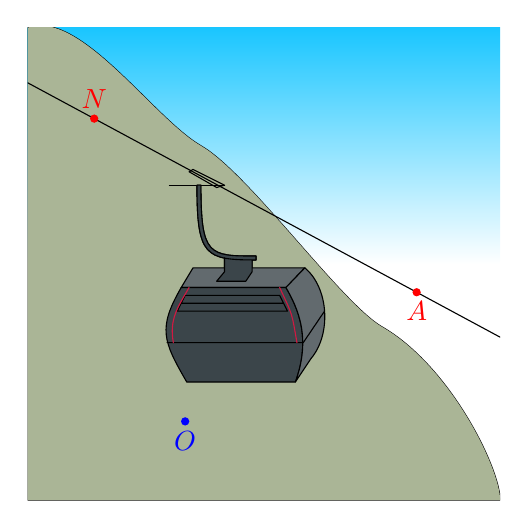
\begin{tikzpicture}[line join=round,line cap=round,scale=1,transform shape]
		 \definecolor{ecru}{rgb}{0.76,0.7,0.5}
		\definecolor{darkolivegreen}{rgb}{0.33,0.42,0.18} 
		\definecolor{deepskyblue}{rgb}{0.0,0.75,1.0} 
		 \definecolor{antiquebrass}{rgb}{0.8,0.58,0.46}
		\definecolor{arsenic}{rgb}{0.23,0.27,0.29} 
		\definecolor{ashgrey}{rgb}{0.7,0.75,0.71}\definecolor{alizarin}{rgb}{0.82,0.1,0.26} 
		\clip (-3,-3) rectangle (3,3); 
		\fill[bottom color=white,top color=deepskyblue!90,middle color=white] (-3,-3) rectangle (3,3); 
		\tikzset{dat/.pic={ 
		\def\N{ 
			 (-3,3)
			..controls +(20:.7) and +(150:.7)..(-.8,1.5) 
			..controls  +(-30:.7) and +(150:.6)..(1.5,-.8)
			..controls  +(-30:1) and +(90:.4)..(3,-3)--(-3,-3)--cycle;
		} 
		 \draw\N;
		 \fill[darkolivegreen!50] \N;
			}} 
		 \tikzset{cap_treo/.pic={
		\def\X{ 
			 (-.85,1)--(-.8,1)
			..controls +(-90:.9)  and +(-180:.6)..(-.1,0.1)--(-.1,.05)
			..controls +(-180:.65) and +(-90:.9)..cycle 
			 (-.15,0.05)--(-.15,-.1)--(-.23,-.22)--(-.6,-.22)--(-.5,-.1)--(-.5,.08);
		} 
		\draw\X; 
		\draw  (-3,2.3)--(3.5,-1.2);
		\draw (-1.2,1)--(-.5,1); 
		\draw (-.5,1)--(-.9,1.2)--(-.95,1.17)--(-.6,.97)--cycle; 
		 \draw[fill=arsenic!80](-.9,-.05)--(.52,-.05)--(.28,-.3)--(-1.05,-.3)--cycle;
		 \def\M{
			 (-.85,1)--(-.8,1)
			..controls +(-90:.9)  and +(-180:.6)..(-.1,0.1)--(-.1,.05)
			..controls  +(-180:.65) and +(-90:.9)..cycle
			 (-.15,0.05)--(-.15,-.1)--(-.23,-.22)--(-.6,-.22)--(-.5,-.1)--(-.5,.08);
		 }
		\fill[arsenic]  \M;
		\draw\M; 
		\def\N{ 
			(-1.05,-.3) 
			..controls +(-120:.6)  and +(120:.6)..(-.98,-1.5)--(.4,-1.5)
			 ..controls +(70:.6) and +(-60:.3)..(.28,-.3)--cycle;
		} 
		\fill[arsenic] \N; 
		\draw\N; 
		 \def\P{
			(.4,-1.5) 
			 ..controls +(70:.6) and +(-60:.3)..(.28,-.3)--(.52,-.05)
			..controls  +(-40:.4) and +(50:.4)..(.6,-1.2)--cycle;
		} 
		\fill[arsenic!80]  \P;
		\draw\P; 
		\draw  (-1.23,-1)--(.5,-1)--(.77,-.6);
		\draw (-1.05,-.5)--(-1,-.4)--(.2,-.4)--(.25,-.5)--cycle 
			 (.25,-.5)--(.3,-.6)--(.3,-.6)--(-1.1,-.6)--(.-1.05,-.5)--cycle;
		\draw[alizarin](.42,-1)..controls +(100:.4) and  +(-65:.4)..(.2,-.3);
		\draw[alizarin](-1.15,-1)..controls +(100:.3) and  +(-120:.3)..(-.95,-.3);
			 }}
		 \path
			(0,0)  pic[scale=1]{dat}
			(0,0) pic[scale=1]{cap_treo}; 
		 \path (-3,2.3)--(3.5,-1.2)
			coordinate[pos=0.13](N) 
			coordinate[pos=0.76](A); 
		\fill[red] (N) circle (1.5pt) node[above]{$N$}; 
		\fill[red] (A)  circle (1.5pt) node[below]{$A$};
		\fill[blue] (-1,-2)  circle (1.5pt) node[below]{$O$};
	\end{tikzpicture}
	 }
	 \loigiai{
		Do  tốc độ của cabin là $10$ m/s nên độ dài $AN=10t$ m.\\
		Do hai vectơ $\overrightarrow{AN}$ và $\overrightarrow{u}$ cùng phương  nên $\overrightarrow{AN}=k\overrightarrow{u}$ với $k$ là số thực dương nào đó.\\
		 Suy ra $\left|\overrightarrow{AN}\right|=k\left|\overrightarrow{u}\right|=k\sqrt{(-8)^2+(-6)^2}=10k$.\\
		Vậy  $t=k$, vì thế $\overrightarrow{AN}=k\overrightarrow{u}=t\overrightarrow{u}=(-8t;-6t;0)$.\\
		Gọi $N(a;b;c) \Rightarrow  \overrightarrow{AN}=(a-10;b-3;c)$.
		 Ta có
		\[ 
		\begin{cases} a-10=-8t \\ b-3=-6t \\ c=0
		\end{cases} \Leftrightarrow \begin{cases} a=10-8t \\ b=3-6t \\ c=0.
	\end{cases}
	 \]
	 Do đó $N(10-8t;3-6t;0)$.\\
	Khoảng cách giữa người quan sát và cabin bằng độ dài  đoạn
	 $$ON=\sqrt{(10-8t)^2+(3-6t)^2}=\sqrt{100t^2-196t+109}.$$
	Ta có  $100t^2-196t+109$ đạt giá trị nhỏ nhất tại $t=\dfrac{196}{2\cdot 100}=\dfrac{49}{50}=0{,}98$ s.
 }
\end{bt}

% nguồn: Phan2_Lop_12_Hinh_hoc_Chuong_5
\begin{bt}%[2H5V2-5]%[ma:09068e2a]
	Trong không gian $Oxyz$. Phương  trình tham số của đường thẳng $d$ đi qua $A(1; 1; 3)$, nằm trong mặt phẳng $(P) \colon x + 2y + z - 6 = 0$ và cắt đường thẳng $\Delta \colon \dfrac{x-1}{1} = \dfrac{y}{1} = \dfrac{z}{2}$ có dạng $\heva{& x=1+at \\ & y=1 \\ & z=3+bt }$. Tính giá trị của biểu thức $M = 2024a - b$.
	 \shortans{2025}
	 \loigiai{
		Gọi $B=\Delta \cap (P)\Rightarrow $  tọa độ điểm $B$ là nghiệm của hệ phương trình\\
		$\heva{& x+2y+z-6=0 \\ & \dfrac{x-1}{1} =  \dfrac{y}{1} = \dfrac{z}{2} } \Leftrightarrow \heva{& x=2 \\ & y=1 \\ & z=2 }\Rightarrow B(2; 1; 2)$.\\
		Vì $d \subset (P)$ và $d$ cắt $\Delta \Rightarrow B \in d\Rightarrow d$ đi qua $A(1;  1; 3)$ và nhận $\vec{AB} = (1; 0; -1)$ làm một VTCP.\\
		Suy ra PTTS của $d \colon \heva{& x=1+t \\ & y=1  \\ & z=3-t} \Rightarrow a=1, b=-1 \Rightarrow M = 2025$.
	 }
\end{bt}

% nguồn: Phan2_Lop_12_Hinh_hoc_Chuong_5
\begin{bt}%[2H5V2-5]%[ma:d60ece1c]
	Trong không gian $Oxyz$, cho mặt phẳng $(\alpha)\colon ax + by + cz + 10 = 0$. Biết  mặt phẳng $(\alpha)$ chứa hai đường thẳng $d \colon \heva{& x=-1+t \\ & y=2+2t \\ & z=-t}$ và $d' \colon \heva{& x=-1+2t' \\ & y=4+2t \\ & z=-1-t }$. Tính $a + b + c$.
	 \shortans{-1}
	 \loigiai{
		Đường thẳng $d$, $d'$ có VTCP lần lượt là $\vec{u}_d =  (1;2;-1)$, $\vec{u_{d'}} = (2; 2; 1)$.\\
		Gọi $A = d \cap d' \Rightarrow \heva{& -1+t=-1+2t' \\ & 2+2t=4+2t \\ & -t=-3-t'} \Leftrightarrow \heva{& t-2t'=0 \\ & 2t-2t'=2 \\ & -t-t'=-3} \Leftrightarrow \heva{& t=2 \\  & t'=1} \Rightarrow A(1; 6; -2)$.\\
		Vì mặt phẳng $(\alpha)$ chứa hai đường thẳng $d$ và $ d'$  nên $(\alpha)$ có VTPT là \break
		$\vec{n}_{(\alpha)} =  \left[\vec{u}_d, \vec{u}_d'\right] = (4; -3; -2)$.\\
		Phương trình mặt phẳng $(\alpha)  \colon 4(x-1)-3(y-6)-2(z+2)=0 \Leftrightarrow 4x - 3y - 2z + 10 = 0$.\\
		Suy ra $a + b +  c= 4 + (-3) + (-2) = -1$.
	} 
\end{bt}

% nguồn: Phan2_Lop_12_Hinh_hoc_Chuong_5
\begin{bt}%[2H5V2-5]%[ma:a54ff842]
	Trong không gian với hệ trục tọa độ $Oxyz$, cho điểm $A(2;1;3)$, mặt phẳng \break$(P)\colon x+y-2z+2=0$ và đường thẳng $d\colon\dfrac{x+1}{1}=\dfrac{y-1}{-2}=\dfrac{z-2}{2}$. Phương trình chính tắc của đường thẳng $\Delta$ đi qua $A$, song song với mặt phẳng $(P)$ và vuông góc với đường thẳng $d$ có dạng $\dfrac{x+a}{b}=\dfrac{y-5}{c}=\dfrac{z+d}{3}$. Giá trị của biểu  thức $M=a+b+c+d$ bằng bao nhiêu?
	 \shortans{-4}
	 \loigiai{
		Ta có $\overrightarrow{n}_{(P)}=(1;1;-2)$ là một vectơ pháp tuyến của mặt phẳng $(P)$ và $\overrightarrow{u}_{d}=(1;-2;2)$ là một  vectơ chỉ phương của đường thẳng $d$.\\
		Do $\Delta$ song song với mặt phẳng $(P)$ và vuông góc với đường thẳng $d$ nên hai vectơ $\overrightarrow{n}_{(P)}$ và $\overrightarrow{u}_{d}$ có giá vuông góc với  đường thẳng $\Delta$.\\
		 Ta có $\overrightarrow{n}_{(P)}$ và $\overrightarrow{u}_{d}$ không cùng phương nên $u=\left[\overrightarrow{n}_{(P)},\overrightarrow{u}_{d}\right]=(-2;-4;-3)$ là một vectơ chỉ phương của đường thẳng $\Delta$.\\
		Khi đó, đường thẳng $\Delta$ đi qua điểm $A(2;1;3)$, nhận $\overrightarrow{u}'=-\overrightarrow{u}=(2;4;3)$ là vectơ  chỉ phương có phương trình chính tắc là
		\begin{eqnarray*}
			 && \dfrac{x-2}{2}=\dfrac{y-1}{4}=\dfrac{z-3}{3} \\
			&\Leftrightarrow&  \dfrac{x-2}{2}-1=\dfrac{y-1}{4}-1=\dfrac{z-3}{3}-1 \\
			&\Leftrightarrow& \dfrac{x-4}{2}=\dfrac{y-5}{4}=\dfrac{z-6}{3}. 
		\end{eqnarray*}
		Suy ra $a=-4$; $b=2$; $c=4$; $d=-6$.\\ 
		Vậy $M=a+b+c+d=(-4)+2+4+(-6)=-4$. 
	} 
\end{bt}

% nguồn: Phan2_Lop_12_Hinh_hoc_Chuong_5
\begin{bt}%[2H5V2-5]%[ma:11faa583]
	Trong không gian $Oxyz$, cho hai đường thẳng $d \colon \dfrac{x-2}{2}= \dfrac{y}{-1} = \dfrac{z}{4}$ và $\Delta \colon \dfrac{x-1}{2} = \dfrac{y-2}{-1} = \dfrac{z+1}{4}$. Phương trình mặt phẳng $(P)$ chứa $d$ và $\Delta$ có dạng $ax + by + z + c =0$. Tính giá trị của $a + b + c$. 
	 \shortans{-2}
	\loigiai{Đường thẳng $d\colon \dfrac{x-2}{2} = \dfrac{y}{-1} = \dfrac{z}{4} \Rightarrow d$ qua $M(2; 0; 0)$ và nhận  $\vec{u} = (2;-1;4)$ làm một VTCP.\\
		Đường thẳng $\Delta \colon  \dfrac{x-1}{2} = \dfrac{y-2}{-1} = \dfrac{z+1}{4} \Rightarrow \Delta $ qua $N(1;2;-1)$ và nhận $\vec{u} = (2; -1; 4)$ làm một VTCP.\\
		Thế tọa độ điểm $M(2;0;0)$  vào đường thẳng $\Delta $, ta được $\dfrac{1}{2}\ne \dfrac{-2}{-1} \ne \dfrac{1}{4} \Rightarrow d \parallel \Delta $.\\
		Khi đó $\vec{MN} = (-1;  2; -1)$.\\
		 $(P)$ chứa $d$ và $\Delta \Rightarrow \vec{n_p} = \left[\vec{u}; \vec{MN}\right] = (7; -7; 7)$.\\
		Suy ra phương trình mặt phẳng $(P) \colon  x - y + z - 2 = 0$.\\
		Khi đó $a = 1$; $b = -1$; $c = -2 \Rightarrow a +  b + c = -2$.
	 }
\end{bt}

% nguồn: Phan2_Lop_12_Hinh_hoc_Chuong_5
\begin{bt}%[2H5V2-5]%[ma:e9373f21]
	Trong không gian với hệ trục tọa độ $Oxyz$, cho điểm $A(2; 1; 3)$ và đường thẳng \break $\Delta \colon \dfrac{x+1}{1} = \dfrac{y-1}{-2} = \dfrac{z-2}{2}$. Gọi $\vec{u}=(a; b; 3)$ là một vectơ chỉ phương của đường thẳng $d$ đi  qua điểm $A$, vuông góc với đường thẳng $\Delta$ và cắt trục $Oy$. Tính $a + b$.
	 \shortans{6}
	 \loigiai{
		Gọi giao điểm của đường thẳng $d$ và trục $Oy$ là $B(0; t; 0)$.\\ 
		Đường thẳng $\Delta$ có vectơ chỉ phương là $\vec{u} = (1; -2; 2)$.\\ 
		Đường thẳng $d$ có vectơ chỉ phương là $\vec{AB} = (-2; t - 1; -3)$.\\ 
		Từ  giả thiết ta có $\vec{u} \perp \vec{AB} \Leftrightarrow \vec{u} \cdot \vec{AB} = 0 \Leftrightarrow -2 - 2(t - 1) - 6 = 0 \Leftrightarrow t = -3$.\\
		Có $\vec{AB} = (-2; -4; -3)$ nên  có thể chọn $\vec{v} = (2; 4; 3)$ là véc tơ chỉ phương của $d$.\\
		Vậy $a = 2$, $b = 4$  nên $a + b = 6$.
	 }
\end{bt}

% nguồn: Phan2_Lop_12_Hinh_hoc_Chuong_5
\begin{bt}%[2H5V2-5]%[ma:36aec41a]
	Trong không gian $Oxyz$, cho mặt phẳng $(\alpha)$ và $B(3; a; 2a)$. Biết mặt phẳng $(\alpha)$ chứa hai đường thẳng $d \colon \heva{& x=-1+5t \\ & y=2-4t \\ & z=3+3t}$ và đường thẳng $d' \colon \heva{& x=2+5t \\ & y=-4t \\ & z=5+3t}$. Khi đó để điểm  $B$ nằm trong mặt phẳng $(\alpha)$ thì giá trị của $a$ bằng
	\shortans{4} 
	\loigiai{ 
		Đường thẳng $d$ có vectơ chỉ phương là $\vec{u} = (5; -4; 3)$ và đi qua  điểm $A(-1; 2; 3)$.\\
		Đường thẳng $d'$ có vectơ chỉ phương là $\vec{u} = (5; -4; 3)$ và đi  qua điểm $B(2; 0; 5)$.\\
		Khi đó $\vec{AB} =  (3; -2; 2)$.\\
		Vì mặt phẳng $(\alpha)$ chứa đường thẳng $d$ và $d'$ nên $(\alpha)$ có VTPT là\\ $\vec{n}_{(\alpha)}= \left[\vec{u}_d,\vec{u_d'}\right]  = (2; 1; -2)$.\\
		Phương trình mặt phẳng $(\alpha)$ có VTPT $\vec{n}_{(\alpha)} = (2; 1; -2)$ và đi qua điểm $A(-1; 2; 3)$ là $$2(x + 1) + (y - 2) - 2(z - 3) = 0 \Leftrightarrow 2x + y - 2z + 6 =  0.$$
		Do $B  \in (\alpha) \Rightarrow 2 \cdot 3 + a - 2 \cdot 2a + 6 = 0 \Leftrightarrow a = 4$.
	} 
\end{bt}

% nguồn: Phan2_Lop_12_Hinh_hoc_Chuong_5
\begin{bt}%[2H5V2-5]%[ma:e02eea67]
	Trong không gian với hệ  tọa độ $Oxyz$, phương trình tham số của đường thẳng $(\Delta)$ qua $M(2; 3; 1)$ và song song với hai mặt phẳng $(P) \colon 2x - y + 2z - 7 = 0$ và $(Q) \colon x + 3y - 2z + 3 = 0$ có dạng $\heva{& x=a+bt \\ & y=3+6t \\ & z=c+dt }; t \in \mathbb{R}$. Tính $2a+b+c+d$.
	 \shortans{8}
	\loigiai{ 
		Mặt phẳng $(P) \colon 2x-y+2z-7=0$ có vectơ pháp tuyến là $\vec{n_1} = (2; -1; 2)$.\\ 
		Mặt phẳng $(Q) \colon x+3y-2z+3 = 0$  có vectơ pháp tuyến là $\vec{n_2} = (1; 3; -2)$.\\
		Vì $(\Delta) \parallel (P)$ và $(\Delta) \parallel (Q)$ nên vectơ chỉ phương của $(\Delta)$ là  $\vec{a} = \left[\vec{n_1}, \vec{n_2}\right] = (-4; 6; 7)$.\\
		Phương trình tham số của đường thẳng $(\Delta) \colon \heva{& x=2-4t \\ & y=3+6t \\ &  z=1+7t} (t \in \mathbb{R})$.\\
		Suy ra $2a+b+c+d  = 8$.
	 }
\end{bt}

% nguồn: Phan2_Lop_12_Hinh_hoc_Chuong_5
\begin{bt}%[2H5V2-5]%[ma:d0b3c158]
	Trong hệ toạ độ $Oxyz$, vào lúc $t=0$ (giờ), một chiến đấu cơ tàng hình Alfa xuất phát từ căn cứ $A_0(0;0;10)$ (đơn vị: km) bắt đầu thực hiện nhiệm vụ tuần tra với véc-tơ vận tốc không đổi $\overrightarrow{v}_A=(800;600;0)$. Cùng lúc đó, một máy bay ném bom Bravo bị phát hiện tại vị trí $B_0(500;0;12)$ đang di chuyển với véc-tơ vận tốc không đổi $\overrightarrow{v}_B=(-400;300;-1)$ hướng về một khu vực mục tiêu được xác định bởi mặt phẳng $(P)\colon z=8$. Để đảm bảo an toàn, căn cứ Alfa có một vùng bán cầu cảnh báo sớm trên không, tâm tại trạm radar mặt đất Omega có tọa độ $R(100;100;0)$ và bán kính $r=150$ km (chỉ xét phần không gian $z \ge 0$). Chiến đấu cơ Alfa  được trang bị tên lửa không đối không thế hệ mới có tốc độ không đổi là $v_M=2\,500$ km/h. Giả sử Alfa quyết định phóng tên lửa vào thời điểm $t_L$ (giờ) để đánh chặn chính xác máy bay Bravo ngay khi Bravo vừa chạm vào mặt phẳng mục tiêu $(P)$. Để đảm bảo tàng hình và tránh bị hệ thống phòng thủ mặt đất phát hiện sớm, Alfa chỉ có thể phóng tên lửa khi nó đang ở \textbf{bên ngoài} vùng bán cầu cảnh báo sớm của trạm Omega. Xác định thời điểm $t_L$ \textbf{muộn nhất} (\textit{tính theo giờ, làm tròn đến $2$ chữ số thập phân}) mà chiến đấu cơ Alfa có thể phóng tên lửa để vừa hoàn thành nhiệm vụ đánh chặn mục tiêu Bravo theo kế hoạch, vừa đảm bảo an toàn cho chính mình theo các điều kiện đã nêu?
	\shortans{2,69} 
	\loigiai{ 
		\textbf{1. Xác định thời điểm và vị trí đánh chặn của Bravo:}\\ 
		Phương trình đường bay của  Bravo theo thời gian $t$ là $B(t)=B_0+t\overrightarrow{v}_B=(500-400t; 300t; 12-t)$.\\
		Bravo  chạm mặt phẳng mục tiêu $(P)\colon z=8$ khi $12-t=8 \Rightarrow t=4$ giờ.\\
		Vị trí đánh chặn là $P=B(4)=(500-400\cdot 4; 300\cdot 4;  12-4)=(-1\,100; 1\,200; 8)$.\\
		\textbf{2. Thiết lập phương trình  đánh chặn:}\\
		Vị trí của Alfa tại thời  điểm phóng tên lửa $t_L$ là\\
		$A(t_L)=A_0+t_L\overrightarrow{v}_A=(800t_L; 600t_L; 10)$. Gọi điểm  này là $N(800t_L; 600t_L; 10)$.\\
		Tên lửa được phóng từ $N$ lúc $t_L$  và đánh chặn Bravo tại $P$ lúc $t=4$.\\
		Thời gian bay của tên lửa là $\Delta t=4-t_L$ (điều kiện  $t_L < 4$).\\
		Quãng đường tên lửa bay được là $d_M=v_M \cdot \Delta  t=2500(4-t_L)$.\\
		 Quãng đường này cũng chính là khoảng cách giữa điểm phóng $N$ và điểm đánh chặn $P$.\\
		 Ta có \allowdisplaybreaks
		\begin{eqnarray*}
			&&NP=d_M\\ 
			&\Leftrightarrow&  \sqrt{(-1\,100-800t_L)^2+(1\,200-600t_L)^2+(8-10)^2}=2\,500(4-t_L)\\
			&\Leftrightarrow&1\,312\,500t_L^2-12\,580\,000t_L+24\,337\,499=0\\ 
			&\Leftrightarrow&\hoac {&t_L \approx 6{,}90\ (\text  {không thoả vì } t_L<4)\\&t_L \approx 2{,}69.}
		\end{eqnarray*}
		Vậy thời điểm phóng tên lửa là $t_L \approx 2{,}69$  giờ.\\
		\textbf{3.  Kiểm tra điều kiện an toàn:}\\
		Alfa tại thời điểm $t_L  \approx 2{,}69$ phải ở bên ngoài vùng bán cầu cảnh báo.\\
		Vị trí của Alfa tại $t_L$ là $N(800 \cdot 2{,}69; 600 \cdot 2{,}69;  10)=N(2\,152; 1614; 10)$.\\
		Tâm radar là $R(100;100;0)$ khi  đó khoảng cách từ Alfa đến tâm radar là
		\[NR=\sqrt{(2\,152-100)^2+(1614-100)^2+(10-0)^2}  \approx 2\,550 \text {km.}\]
		Vì $NR \approx 2\,550$ km $> 150$ km (bán kính vùng cảnh báo), điều  kiện an toàn được thỏa mãn.\\ Thời điểm $t_L$ muộn nhất là $t_L \approx 2{,}69$ giờ.\\
	} 
\end{bt}


%%%%%%%%%%%%%%%% TỰ LUẬN %%%%%%%%%%%%%%%%

% nguồn: Phan2_Lop_12_Hinh_hoc_Chuong_5
\begin{bt}%[2H5H2-5]%[ma:7628247b]
	Trong không gian $Oxyz$, cho điểm $M(3;1;-2)$ và mặt  phẳng $(P)\colon 3x+5y-z+1=0$. Viết phương trình đường thẳng đi qua $M$ và vuông góc $(P)$.
	 \loigiai{
		Mặt phẳng $(P)$ có một vectơ pháp  tuyến là $\overrightarrow{n}_P=(3;5;-1)$.\\
		Gọi $d$ là đường thẳng đi  qua $M$ và vuông góc $(P)$.\\
		Vì $d$ vuông góc $(P)$ nên nhận vectơ $\overrightarrow{n}_P=(3;5;-1)$ làm vectơ chỉ  phương.\\
		Vậy phương trình đường thẳng $d$ là $\dfrac{x-3}{3}=\dfrac{y-1}{5}=\dfrac{z+2}{-1}$. 
	} 
\end{bt}

% nguồn: Phan2_Lop_12_Hinh_hoc_Chuong_5
\begin{bt}%[2H5H2-5]%[ma:cc034eee]
	Trong không gian với hệ toạ độ $Oxyz$, viết các phương trình tham số và chính tắc của đường thẳng $\Delta$ đi qua $A(2;-1;4)$ và vuông  góc với mặt phẳng $(P) \colon x+3y-z-1=0$.
	\loigiai{ 
		 Mặt phẳng $(P)$ có vectơ pháp tuyến là $\overrightarrow{n}=(1;3;-1)$. \\
		Vì $\Delta \perp (P)$ nên vectơ chỉ phương của $\Delta$  là $\overrightarrow{u}=\overrightarrow{n}=(1;3;-1)$. \\
		Đường thẳng  $\Delta$ đi qua điểm $A(2;-1;4)$ và có vectơ chỉ phương là $\overrightarrow{u}=(1;3;-1)$. \\
		Phương  trình tham số của $\Delta$ là
		$\heva{ 
		 &x=2+t \\
		&y=-1+3t  \\
		 &z=4-t
		} \quad  (t \in \mathbb{R})$. \\
		Phương trình chính tắc của $\Delta$ là 
		 $\dfrac{x-2}{1}=\dfrac{y+1}{3}=\dfrac{z-4}{-1}$.
	} 
\end{bt}

% nguồn: Phan2_Lop_12_Hinh_hoc_Chuong_5
\begin{bt}%[2H5H2-5]%[ma:5e2d533e]
	Trong  không gian $Oxyz$, cho điểm $A(0;2;-4)$ và đường thẳng $d\colon \dfrac{x-2}{1}=\dfrac{y-1}{-1}=\dfrac{z+1}{2}$. Tìm tọa độ hình chiếu $H$ của $A$ xuống $d$.
	 \loigiai{
		Xét mặt phẳng $(P)$ đi qua $A$ và vuông góc với đường thẳng $d$ nên mặt phẳng $(P)$ đi qua $A(0;2;4)$  và có vectơ pháp tuyến $\overrightarrow{n}_P=\overrightarrow{u}=(1;-1;2)$.\\
		Phương trình mặt phẳng $(P)$  là $(x-0)-1(y-2)+2(z+4)=0\Leftrightarrow x-y+2z+10=0$.\\
		Hình chiếu  $H$ của $A$ xuống $d$ là giao điểm của $(P)$ và đường thẳng $d$, tọa độ điểm $H$ là nghiệm của hệ phương trình
		\[\heva{&x-y+2z+10=0\\ 
		 &x+y-3=0\\
		&2x-z-5=0} 
		\Rightarrow\heva{&x=\dfrac{1}{2}\\ 
		 &y=\dfrac{5}{2}\\
		 &z=-4.}\]
		Vậy tọa độ hình chiếu là $H\left(\dfrac{1}{2};\dfrac{5}{2};-4\right)$. 
	} 
\end{bt}

% nguồn: Ok_TuanLuan_Toan11_Lan2
\begin{ex}%[2H5V2-5]%[ma:9e69bd06]
	Cho hình tứ diện $EFGH$ có $EF$ vuông góc với $EG$, $EG$ vuông góc với $EH$, $EH$ vuông góc với $EF$. Biết $EF = 6a$, $EG = 8a$, $EH = 12a$ (với $a > 0, a \in \mathbb{R}$). Gọi $I, J$ tương ứng là trung điểm của hai cạnh $FG, FH$. Tính khoảng cách $d$ từ điểm $F$ đến mặt phẳng $(EIJ)$  theo $a$.
	 \loigiai{
		Vì $EF \perp EG$, $EG \perp EH$, $EH \perp EF$ nên tam giác  $EFH$ vuông tại $F$.\\
		Gọi $K$ là  trung điểm của $EF$ suy ra $IK \perp (EFH)$.\\
		Chọn hệ tọa độ $Oxyz$ như  hình vẽ. Khi đó ta có
		 $
		K(0;0;0)$, $I(0;0;4a)$,  $E(3a;0;0)$, $ J(0;6a;0)$.
		\begin{center}
			 \tdplotsetmaincoords{70}{110}
			\begin{tikzpicture}[tdplot_main_coords,scale=0.8]
					\pgfmathsetmacro{\a}{1} 
					\coordinate (K) at  (0,0,0);
					 \coordinate (E) at (4*\a,0,0);
					\coordinate (J)  at (-0.5,6*\a,0);
					\coordinate (I) at (0,0,4*\a); 
						 midpoints I,J)
					\coordinate (F) at (-4*\a,0,0); 
					\coordinate (G)  at (4*\a,0,8*\a);
					\coordinate (H)  at (3*\a,12*\a,0);
					 \coordinate (M) at (1.5*\a,3*\a,0);
					\coordinate  (N) at (1.5*\a,0,2*\a);
					\draw[->] (4*\a,0,0) --  (6*\a,0,0) node[right] {$x$};
					\draw[->] (-0.5,6*\a,0)  -- (-0.7,8*\a,0) node[above] {$y$};
					 \draw[->] (0,0,4*\a) -- (0,0,6*\a) node[left] {$z$};
					\draw(E) --  (G);
					\draw(E) -- (H); 
					 \draw(G) -- (H);
					 \draw[dashed] (E) -- (F);
					\draw[dashed]  (F) -- (G);
					\draw[dashed] (F)  -- (H);
					\draw[dashed] (K)  -- (E);
					\draw[dashed] (K)  -- (J);
					\draw[dashed] (K) --  (I);
					\draw[dashed] (E) -- (M); 
					\draw[dashed] (E) -- (N); 
					\draw[dashed]  (J) -- (M);
					\draw[dashed] (M)  -- (I) -- (N);
					\draw[dashed]  (K) -- (M) -- (N);
					\foreach  \point/\pos in {K/below,E/below right,I/left,J/below,
						F/above right,G/above  left,H/below right,M/below right,N/above left}
					\fill (\point) circle  (1pt) node[\pos] {$\point$};
					\node at  ($(E)!0.5!(G)$) [left] {$8a$};
					\node  at ($(E)!0.5!(H)$) [below] {$12a$};
					\draw (E) -- ($(E) + (-0.5*\a,0,0)$) -- ($(E) + (-0.5*\a,0,0)  + (0,0,0.5*\a)$) -- ($(E) + (0,0,0.5*\a)$) -- cycle;
					\draw (E) -- ($(E) + (-0.5*\a,0,0)$) -- ($(E) + (-0.5*\a,0,0) + (0,0.5*\a,0)$) -- ($(E) +  (0,0.5*\a,0)$) -- cycle;
					\draw (E) -- ($(E) + (0,0,0.5*\a)$) -- ($(E)  + (0,0,0.5*\a) + (0,0.5*\a,0)$) -- ($(E) + (0,0.5*\a,0)$) -- cycle;
				\end{tikzpicture}
		\end{center}
		Phương  trình mặt phẳng $(EIJ)$ qua 3 điểm $
		 E(3a;0;0)$, $ I(0;0;4a) $, $ J(0;6a;0)$
		 có dạng
		$$ 
		\dfrac{x}{3a} + \dfrac{y}{6a} + \dfrac{z}{4a} = 1 \Leftrightarrow 4x + 2y  + 3z - 12a = 0.
		 $$
		Vì $F(0;6a;0)$,  ta có
		 $$
		\mathrm{d}(F,(EIJ)) = 2 \cdot \mathrm{d}(K,(EIJ)) = 2 \cdot \dfrac{\left|4 \cdot  0 + 2 \cdot 0 + 3 \cdot 0 - 12a\right|}{\sqrt{4^2 + 2^2 + 3^2}} = \dfrac{24a}{\sqrt{29}} = \dfrac{24\sqrt{29}a}{29}.
		$$ 
	} 
\end{ex}

% nguồn: Phan2_Lop_12_Hinh_hoc_Chuong_5
\begin{bt}%[2H5V2-5]%[ma:ccb6a67d]
	Cho hình tứ diện $EFGH$ có $EF$ vuông góc với $EG$, $EG$ vuông góc với $EH$, $EH$ vuông góc với $EF$. Biết $EF = 6a$, $EG = 8a$, $EH = 12a$  (với $a > 0, a \in \mathbb{R}$). Gọi $I, J$ tương ứng là trung điểm của hai cạnh $FG, FH$. Tính khoảng cách $d$ từ điểm $F$ đến mặt phẳng $(EIJ)$ theo $a$.
	 \loigiai{
		Vì $EF \perp EG$, $EG \perp EH$, $EH \perp EF$  nên tam giác $EFH$ vuông tại $F$.\\
		Gọi $K$ là trung điểm của $EF$ suy ra $IK \perp  (EFH)$.\\
		Chọn  hệ tọa độ $Oxyz$ như hình vẽ. Khi đó ta có
		$ 
		K(0;0;0)$, $I(0;0;4a)$, $E(3a;0;0)$, $  J(0;6a;0)$.
		\begin{center}
			\tdplotsetmaincoords{70}{110} 
			\begin{tikzpicture}[tdplot_main_coords,scale=0.8]
					 \pgfmathsetmacro{\a}{1}
					\coordinate  (K) at (0,0,0);
					 \coordinate (E) at (4*\a,0,0);
					\coordinate (J) at  (-0.5,6*\a,0);
					\coordinate (I) at  (0,0,4*\a);
						midpoints I,J) 
					\coordinate (F) at (-4*\a,0,0); 
					 \coordinate (G) at (4*\a,0,8*\a);
					\coordinate  (H) at (3*\a,12*\a,0);
					\coordinate (M) at (1.5*\a,3*\a,0); 
					\coordinate  (N) at (1.5*\a,0,2*\a);
					\draw[->] (4*\a,0,0)  -- (6*\a,0,0) node[right] {$x$};
					 \draw[->] (-0.5,6*\a,0) -- (-0.7,8*\a,0) node[above] {$y$};
					\draw[->] (0,0,4*\a) -- (0,0,6*\a)  node[left] {$z$};
					 \draw (E) -- (G);
					\draw  (E) -- (H);
					\draw  (G) -- (H);
					\draw[dashed]  (E) -- (F);
					 \draw[dashed] (F) -- (G);
					\draw[dashed] (F)  -- (H);
					\draw[dashed] (K) -- (E); 
					\draw[dashed] (K) -- (J); 
					\draw[dashed] (K)  -- (I);
					\draw[dashed]  (E) -- (M);
					 \draw[dashed] (E) -- (N);
					 \draw[dashed] (J) -- (M);
					 \draw[dashed] (M) -- (I) -- (N);
					\draw[dashed] (K) -- (M) --  (N);
					\foreach \point/\pos in  {K/below,E/below right,I/left,J/below,
						F/above right,G/above left,H/below right,M/below right,N/above left} 
					\fill (\point) circle  (2pt) node[\pos] {$\point$};
					\node  at ($(E)!0.5!(G)$) [left] {$8a$};
					\node at ($(E)!0.5!(H)$) [below] {$12a$}; 
					\draw (E) -- ($(E) + (-0.5*\a,0,0)$) -- ($(E) +  (-0.5*\a,0,0) + (0,0,0.5*\a)$) -- ($(E) + (0,0,0.5*\a)$) -- cycle;
					\draw (E) -- ($(E) + (-0.5*\a,0,0)$) -- ($(E) + (-0.5*\a,0,0) +  (0,0.5*\a,0)$) -- ($(E) + (0,0.5*\a,0)$) -- cycle;
					\draw (E)  -- ($(E) + (0,0,0.5*\a)$) -- ($(E) + (0,0,0.5*\a) + (0,0.5*\a,0)$) -- ($(E) + (0,0.5*\a,0)$) -- cycle;
				\end{tikzpicture}
		\end{center}
		Phương trình mặt phẳng $(EIJ)$ qua 3  điểm $
		E(3a;0;0)$, $ I(0;0;4a)  $, $ J(0;6a;0)$
		có dạng 
		 $$
		\dfrac{x}{3a} + \dfrac{y}{6a} + \dfrac{z}{4a} = 1 \Leftrightarrow 4x + 2y + 3z -  12a = 0.
		 $$
		Vì $F(0;6a;0)$, ta có 
		$$ 
		\mathrm{d}(F,(EIJ)) = 2 \cdot \mathrm{d}(K,(EIJ)) = 2 \cdot \dfrac{\left|4 \cdot 0 + 2 \cdot 0 + 3 \cdot 0 -  12a\right|}{\sqrt{4^2 + 2^2 + 3^2}} = \dfrac{24a}{\sqrt{29}} = \dfrac{24\sqrt{29}a}{29}.
		 $$
	} 
\end{bt}
